\documentclass[letterpaper]{article}
\usepackage[margin=1in]{geometry}
\usepackage[utf8]{inputenc}
\usepackage{textcomp}
\usepackage{amssymb}
\usepackage{natbib}
\usepackage{graphicx}
\usepackage{gensymb}
\usepackage{amsthm, amsmath, mathtools}
\usepackage[dvipsnames]{xcolor}
\usepackage{enumerate}
\usepackage{mdframed}
\usepackage[most]{tcolorbox}
\usepackage{csquotes}
% https://tex.stackexchange.com/questions/13506/how-to-continue-the-framed-text-box-on-multiple-pages

\tcbuselibrary{theorems}

\newcommand{\R}{\mathbb{R}}
\newcommand{\Z}{\mathbb{Z}}
\newcommand{\N}{\mathbb{N}}
\newcommand{\Q}{\mathbb{Q}}
\newcommand{\C}{\mathbb{C}}
\newcommand{\code}[1]{\texttt{#1}}
\newcommand{\mdiamond}{$\diamondsuit$}
\newcommand{\PowerSet}{\mathcal{P}}
\newcommand{\Mod}[1]{\ (\mathrm{mod}\ #1)}
\DeclareMathOperator{\lcm}{lcm}

%\newtheorem*{theorem}{Theorem}
%\newtheorem*{definition}{Definition}
%\newtheorem*{corollary}{Corollary}
%\newtheorem*{lemma}{Lemma}
\newtheorem*{proposition}{Proposition}


\newtcbtheorem[number within=section]{theorem}{Theorem}
{colback=green!5,colframe=green!35!black,fonttitle=\bfseries}{th}

\newtcbtheorem[number within=section]{definition}{Definition}
{colback=blue!5,colframe=blue!35!black,fonttitle=\bfseries}{def}

\newtcbtheorem[number within=section]{corollary}{Corollary}
{colback=yellow!5,colframe=yellow!35!black,fonttitle=\bfseries}{cor}

\newtcbtheorem[number within=section]{lemma}{Lemma}
{colback=red!5,colframe=red!35!black,fonttitle=\bfseries}{lem}

\newtcbtheorem[number within=section]{example}{Example}
{colback=white!5,colframe=white!35!black,fonttitle=\bfseries}{def}

\newtcbtheorem[number within=section]{note}{Important Note}{
        enhanced,
        sharp corners,
        attach boxed title to top left={
            xshift=-1mm,
            yshift=-5mm,
            yshifttext=-1mm
        },
        top=1.5em,
        colback=white,
        colframe=black,
        fonttitle=\bfseries,
        boxed title style={
            sharp corners,
            size=small,
            colback=red!75!black,
            colframe=red!75!black,
        } 
    }{impnote}
\usepackage[utf8]{inputenc}
\usepackage[english]{babel}
\usepackage{fancyhdr}
\usepackage[hidelinks]{hyperref}

\pagestyle{fancy}
\fancyhf{}
\rhead{Math 187A}
\chead{March 12th, 2023}
\lhead{Course Notes}
\rfoot{\thepage}

\setlength{\parindent}{0pt}

\newcommand{\0}{\mathbf{0}}
\newcommand{\y}{\mathbf{y}}
\renewcommand{\b}{\mathbf{b}}
\newcommand{\x}{\mathbf{x}}
\newcommand{\e}{\mathbf{e}}
\newcommand{\rr}{\mathbf{r}}
\newcommand{\vv}{\mathbf{v}}
\renewcommand{\u}{\mathbf{u}}

\begin{document}

\begin{titlepage}
    \begin{center}
        \vspace*{1cm}
            
        \Huge
        \textbf{Math 187A Notes}
            
        \vspace{0.5cm}
        \LARGE
        Introduction to Cryptography
            
        \vspace{1.5cm}
            
        \vfill
            
        Winter 2023\\
        Taught by Professor Shishir (Sunny) Agrawal
    \end{center}
\end{titlepage}

\pagenumbering{gobble}

\newpage 

\pagenumbering{gobble}
\begingroup
    \renewcommand\contentsname{Table of Contents}
    \tableofcontents
\endgroup

\newpage
\pagenumbering{arabic}

\section{Introduction to Cryptography}
We begin with some common definitions.

\subsection{Terminology}
\begin{definition}{Cipher}{}
    A \textbf{cipher}, or cryptosystem, is a cryptographic method for confidential communication. 
\end{definition}
Generally, a cryptographic method includes algorithms for \emph{encryption} and \emph{decryption}, which are inverse processes that convert between plainly readable information called \emph{plaintext}\footnote{In cryptography, we use \emph{plaintext} and \emph{ciphertext} instead of \emph{plain text} and \emph{cipher text}.} and unintelligible information called \emph{ciphertext}.

\begin{definition}{Sender}{}
    A \textbf{sender}, often named ``Alice'' in abstract cryptographic discussions, \emph{encrypts} her plaintext into ciphertext. 
\end{definition}

\begin{definition}{Receiver}{}
    A \textbf{receiver}, often named ``Bob,'' \emph{decrypts} (or deciphers) the ciphertext back into plaintext. 
\end{definition}
Often times, Bob will use a \emph{key} to decrypt the message. This is sometimes known as a private key or decryption key.

\begin{definition}{Encoding}{}
    The (usually) preliminary step where a message is converted into a format which can then be encrypted is called \textbf{encoding}. 
\end{definition}
Note that encoded text is not secure; it is only secure after encryption. So, we can think of encoding as the pre-processing step. In other words, before we encrypt something, we might \emph{encode} the text so it's easier to encrypt. It should also be noted that if a message had to be encoded before encryption, then it will also need to be decoded after decryption. 

\begin{center}
    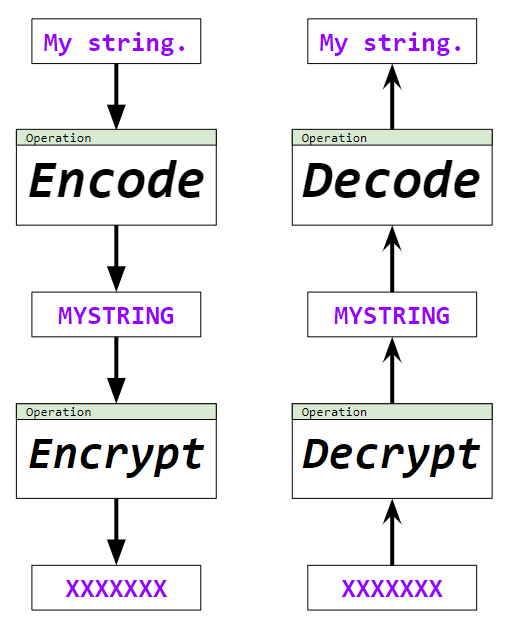
\includegraphics[scale=0.8]{assets/encode_encrypt.png}
\end{center}

\begin{definition}{Adversary}{}
    An \textbf{adversary}, often named ``Eve,'' is one whose aim is to prevent the users of a cryptosystem from achieving their goal. 
\end{definition}
In our case here, an adversary can intercept a ciphertext. Thus, the adversary will not have Bob's decryption key at the beginning. The idea is that, even if the adversary knows what cryptosystem was used to encrypt the message, if the adversary doesn't have this decryption key, she should ideally not be able to decrypt the message. If she does manage to figure out the plaintext, she has \emph{broken} the code.

\begin{definition}{Attack Model}{}
    An \textbf{attack model} specifies what Eve is allowed to do in order to break the code. 
\end{definition}
Some common attack models includes:
\begin{itemize}
    \item Ciphertext-only attack: Eve must recover the plaintext using only the ciphertext.
    \item Known-plaintext attack: Eve may have access to some information about the plaintext (e.g., knowledge of portions of the plaintext), which can be used to recover the plaintext entirely. 
    \item Chosen-plaintext attack: Eve can request or generate ciphertexts corresponding to any plaintext message of her choosing, and she can use this information to recover the plaintext.
\end{itemize}
Classical cryptography was mostly concerned with assuring security against the first two. Modern cryptography tries to assure security against the last. 


\newpage 
\section{Classical Cryptosystems}
We begin with a definition: 
\begin{definition}{$n$-gram}{}
    An $n$-gram is a sequence of $n$ letters.
\end{definition}
For example, a 1-gram is just a single letter; a 2-gram (i.e., \emph{bigram}) is a pair of letters; and so on. Generally, we can group many classical cryptosystems into a few different encryption strategies.

\begin{center}
    \begin{tabular}{|p{1in}|p{5in}|}
        \hline
        \textbf{Strategy} & \textbf{Description} \\ 
        \hline 
        Transposition & Involves rearranging units of plaintext according to some pattern. We'll see just one example of this type of cipher: rectangular transposition. \\ 
        \hline 
        Substitution & Involves replacing units of plaintext with units of ciphertext. We can further group substitution ciphers into some subtypes: 
        \begin{center}
            \begin{tabular}{|p{1in}|p{3.5in}|}
                \hline
                \textbf{Subtype} & \textbf{Description} \\ 
                \hline
                Simple \\ Substitution & In these ciphers, single letters of plaintext are replaced by ciphertext. The substitution scheme stays the same over the course of the entire message. Some examples we'll see include:
                \begin{itemize}
                    \item Masonic cipher 
                    \item Caesar cipher 
                    \item Affine cipher 
                    \item Polybius square 
                \end{itemize}
                In essence, though, there is a 1-1 relationship between the letters of the plaintext and the ciphertext alphabets. \\
                \hline 
                Polygraphic \\ Substitution & In these ciphers, groups of letters in the plaintext are replaced by ciphertext (a group of $n$ letters is called an $n$-gram).The substitution scheme stays the same over the entire message. Some examples we'll see include: 
                \begin{itemize}
                    \item Hill cipher
                    \item Playfair cipher
                \end{itemize}
                So, in essence, polygraphic substitution is just simple substitution but with \emph{groups of letters} instead of individual letters. \\ 
                \hline 
                Polyalphabetic \\ Substitution & In these ciphers, single letters in the plaintext are replaced by ciphertext, and the substitution scheme changes over the course of the message. Some examples include: 
                \begin{itemize}
                    \item Vignere cipher 
                    \item One-time pad 
                \end{itemize} 
                \\ 
                \hline 
            \end{tabular}
        \end{center}
        In practice, however, most cryptosystems employ a combination of these strategies. \\
        \hline 
    \end{tabular}
\end{center}


















\subsection{Rectangular Tranposition}
\textbf{Rectangular tranposition}, known also as \emph{regular columnar transposition}, is a tranposition cipher. The ciphertext is obtained by \emph{permuting} the letters of the plaintext in a particular pattern. The pattern is determined by a secret \emph{keyword}. 

\bigskip 

Roughly speaking, the steps to perform rectangular transposition are as follows:
\begin{enumerate}
    \item Using the keyword, rank the letters based on alphabetical ranking. 
    \item Break up the message into groups of $n$, where $n$ is the length of the keyword.
    \item For each group, do the following: 
    \begin{itemize}
        \item Encrypting: If the $i$th letter of the keyword has rank $j$, move the $i$th letter in the group into the $j$th position.
        \item Decrypting: If the $i$th letter of the keyword has rank $j$, move the $j$th letter of each group into the $i$th position. 
    \end{itemize}
\end{enumerate}
Note that keywords with repeat letters do not work by themselves. We either need to agree not to use words with repeat letters, or remove duplicate letters from the keyword\footnote{In this course, we won't consider words with repeat letters.}.

\begin{mdframed}[]
    (Example: Encryption.) Suppose that Alice and Bob share the keyword \code{GUARD}, and that Alice wants to send the following message to Bob: 
    \begin{mdframed}
        \begin{verbatim}
Hide! The baboons are coming for you. \end{verbatim}
    \end{mdframed}

    First, we'll \textbf{encode} the message so that it's easier to encrypt. In our example, we'll remove all spaces and punctuation. 
    \begin{mdframed}
        \begin{verbatim}
HIDETHEBABOONSARECOMINGFORYOU \end{verbatim}
    \end{mdframed}
    Now that encoding is done, we still need to encrypt the message. Notice how the keyword \code{GUARD} has 5 letters; we can break the message up into 5-grams and then stack them into rows:
    \begin{mdframed}
        \begin{verbatim}
HIDET
HEBAB
OONSA
RECOM
INGFO
RYOU\end{verbatim}
    \end{mdframed}
    We then need to insert some random letters at the end of the message so every row has an equal number of letters. Let's use \code{Q}:
    \begin{mdframed}
        \begin{verbatim}
HIDET
HEBAB
OONSA
RECOM
INGFO
RYOUQ\end{verbatim}
    \end{mdframed}
    Now, we begin the \textbf{encryption} process by rearranging the letters in each row based on the alphabetical ranking of the letters of the keyword \code{GUARD}. 
    \begin{center}
        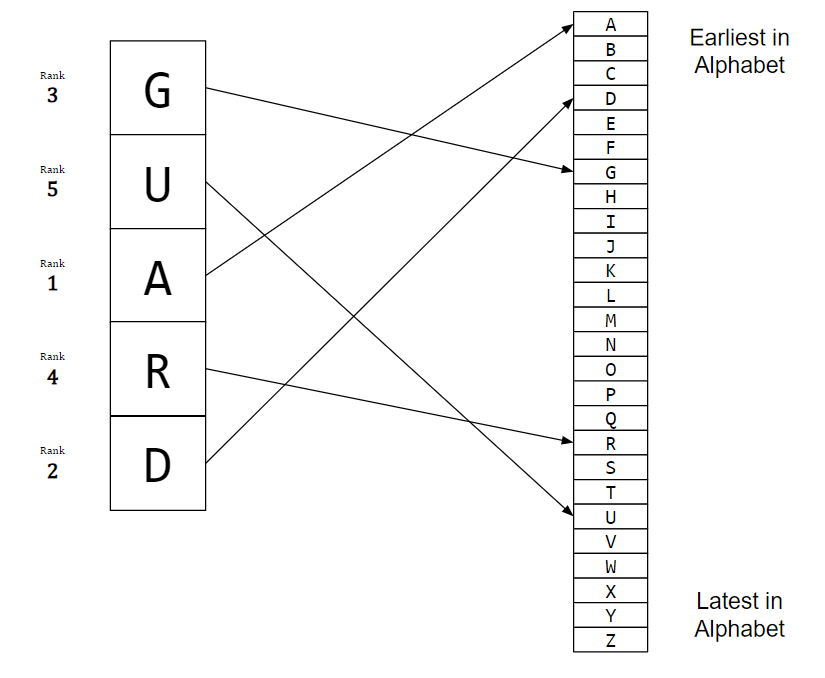
\includegraphics[scale=0.7]{assets/rank_crypto.png}
    \end{center}
    We note that the alphabetical rankings of the letters of this keyword are 3, 5, 1, 4, 2. We can see this as a \emph{permutation}; that is, 
    \[1 \mapsto 3 \qquad 2 \mapsto 5 \qquad 3 \mapsto 1 \qquad 4 \mapsto 4 \qquad 5 \mapsto 2\]
    \textbf{The idea for encryption is that, for each column $i$, we'll send that column to whatever is mapped by the permutation above.} Going back to the stack of letters we have, we can label each individual column:
    \begin{mdframed}
        \begin{verbatim}
plaintext 
position    1 2 3 4 5
            H I D E T
            H E B A B
            O O N S A
            R E C O M
            I N G F O
            R Y O U Q\end{verbatim}
    \end{mdframed}
    The idea is that 
    \begin{itemize}
        \item we can put all letters under position 1 in the plaintext stack to position \textbf{3} of the ciphertext stack, 
        \item we can put all letters under position 2 in the plaintext stack to position \textbf{5} of the ciphertext stack, 
        \item we can put all letters under position 3 in the plaintext stack to position \textbf{1} of the ciphertext stack, 
        \item we can put all letters under position 4 in the plaintext stack to position \textbf{4} of the ciphertext stack, 
        \item we can put all letters under position 5 in the plaintext stack to position \textbf{2} of the ciphertext stack.
    \end{itemize}
    The process, visually, would look like: 
    \begin{center}
        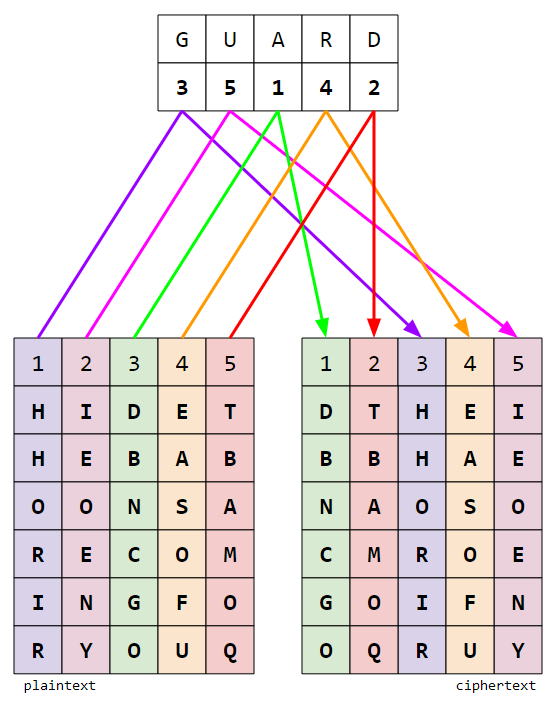
\includegraphics[scale=0.7]{assets/trans_encrypt.png}
    \end{center}
    Therefore, the ciphertext stack would look like: 
    \begin{mdframed}
        \begin{verbatim}
DTHEI
BBHAE
NAOSO
CMROE
GOIFN
OQRUY\end{verbatim}
    \end{mdframed}
    Undoing the stacking gives us the ciphertext: 
    \begin{mdframed}
        \begin{verbatim}
DTHEIBBHAENAOSOCMROEGOIFNOQRUY\end{verbatim}
    \end{mdframed}
\end{mdframed}
\textbf{Remark:} An easy way to run through the process is to create two ``groups,'' side-by-side. The first group will be the plaintext stack, and the second group will be the ciphertext text. Then, label each column of the first group with the \textbf{alphabetical ranking} of the keyword. Label each column of the second group with \textbf{12345}. Finally, map each column from the first group to the second group based on the label. 
\begin{center}
    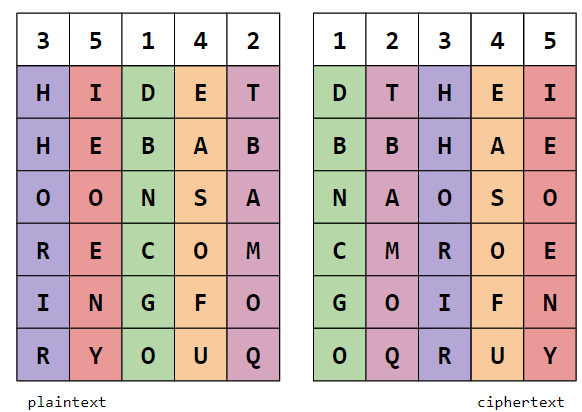
\includegraphics[scale=0.7]{assets/trans_encrypt2.png}
\end{center} 

Decrypting is merely the inverse of the encryption process.
\begin{mdframed}
    (Example: Decryption.) Consider the above example again. Suppose Alice successfully sends the following ciphertext to Bob:
    \begin{mdframed}
        \begin{verbatim}
DTHEIBBHAENAOSOCMROEGOIFNOQRUY\end{verbatim}
    \end{mdframed}
    Bob knows that the keyword is \code{GUARD}. He can use this keyword to decrypt the message. He can begin by taking the letters of the ciphertext and stacking them into rows of 5, since \code{GUARD} has 5 letters:
    \begin{mdframed}
        \begin{verbatim}
DTHEI
BBHAE
NAOSO
CMROE
GOIFN
OQRUY\end{verbatim}
    \end{mdframed}
    Bob also knows the alphabetical ranking of the letters of \code{GUARD} (which is the same rankings as described above). In particular, the alphabetical ranking is \code{35142}. So, we need to do the following: 
    \begin{itemize}
        \item The letters in position 1 of the ciphertext stack needs to be moved to position \textbf{3},
        \item the letters in position 2 of the ciphertext stack needs to be moved to position \textbf{5},
        \item the letters in position 3 of the ciphertext stack needs to be moved to position \textbf{1},
        \item the letters in position 4 of the ciphertext stack needs to be moved to position \textbf{4},
        \item the letters in position 5 of the ciphertext stack needs to be moved to position \textbf{2}. 
    \end{itemize}
    
    The process, visually, would look like: 
    \begin{center}
        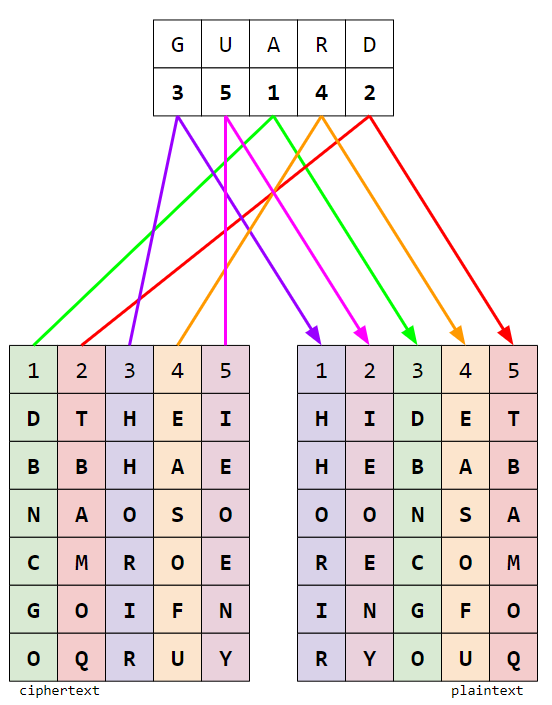
\includegraphics[scale=0.7]{assets/trans_decrypt.png}
    \end{center}
    Undoing the stacking gives us:
    \begin{mdframed}
        \begin{verbatim}
HIDETHEBABOONSARECOMINGFORYOUQ\end{verbatim}
    \end{mdframed}
    At this point, Bob needs to make an educated guess as to what the encoded message says (recall that we had to encode the message before encrypting it). By removing the \code{Q} and correctly punctuating the message, we get 
    \begin{mdframed}
        \begin{verbatim}
Hide! The baboons are coming for you.\end{verbatim}
    \end{mdframed}
\end{mdframed}
\textbf{Remark:} We can easily decrypt an encrypted word by doing the inverse of what we did above. Create two ``groups,'' side-by-side. The first group will be the ciphertext stack, and the second group will be the plaintext text. Then, label each column of the first group with \textbf{12345}. Label each column of the second group with the \textbf{alphabetical ranking} of the keyword. Finally, map each column from the first group to the second group based on the label. 
\begin{center}
    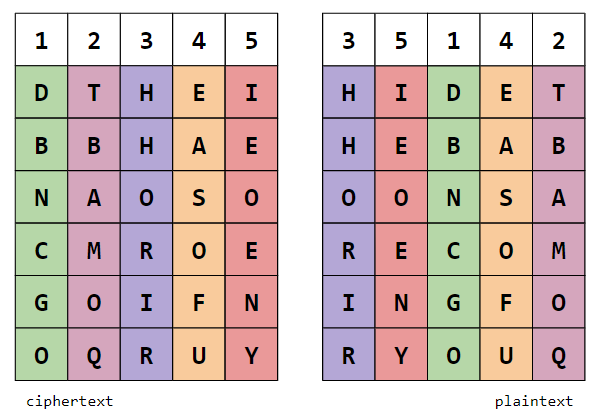
\includegraphics[scale=0.7]{assets/trans_decrypt2.png}
\end{center} 

\begin{mdframed}[]
    (Exercise: Encryption.) \emph{Encrypt the message \code{There is always hope.} using the keyword \code{CRASH}.}

    \begin{mdframed}
        First, we encode the message so that we can easily encrypt it: 
        \begin{mdframed}
            \begin{verbatim}
THEREISALWAYSHOPE\end{verbatim}
        \end{mdframed}

        Noting that \code{CRASH} has length 5, we break the now encoded message into groups of 5 letters (5-grams):
        \begin{mdframed}
            \begin{verbatim}
THERE
ISALW
AYSHO
PE\end{verbatim}
        \end{mdframed}
        
        Let's now add nonsense letters at the end of the last row so every row has 5 letters: 
        \begin{mdframed}
            \begin{verbatim}
THERE
ISALW
AYSHO
PEABC\end{verbatim}
        \end{mdframed}

        Now, we note the alphabetical ranking of each letter in \code{CRASH}:
        \[C \mapsto 2 \quad R \mapsto 4 \quad A \mapsto 1 \quad S \mapsto 5 \quad H \mapsto 3.\]
        Using the streamlined way discussed above, we have 
        \begin{mdframed}
            \begin{verbatim}
2 4 1 5 3 | 1 2 3 4 5
T H E R E | E T E H R
I S A L W | A I W S L
A Y S H O | S A O Y H
P E A B C | A P C E B\end{verbatim}
        \end{mdframed}
        Unstacking the new rows gives us the ciphertext:
        \begin{mdframed}
            \begin{verbatim}
ETEHRAIWSLSAOYHAPCEB\end{verbatim}
        \end{mdframed}
    \end{mdframed}
\end{mdframed}


\begin{mdframed}[nobreak=true]
    (Exercise: Decryption.) \emph{Decrypt the message \code{ETIHGFREAFRSLAESOXOE} using the keyword \code{CRASH}.}

    \begin{mdframed}
        Begin by grouping the letters into 5-grams, since \code{CRASH} has length 5:
        \begin{mdframed}
            \begin{verbatim}
ETIHG
FREAF
RSLAE
SOXOE\end{verbatim}
        \end{mdframed}
        Recall that the alphabetical ranking of each letter in \code{CRASH} is \code{24153}. Using the streamlined way discussed above, we have 
        \begin{mdframed}
            \begin{verbatim}
1 2 3 4 5    2 4 1 5 3
E T I H G -> T H E G I 
F R E A F -> R A F F E 
R S L A E -> S A R E L 
S O X O E -> O O S E X \end{verbatim}
        \end{mdframed}
        Unstacking the new rows gives us the plaintext:
        \begin{mdframed}
            \begin{verbatim}
THEGIRAFFESARELOOSEX\end{verbatim}
        \end{mdframed}
        Decoding the message gives us: 
        \begin{mdframed}
            \begin{verbatim}
The giraffes are loose.\end{verbatim}
        \end{mdframed}
    \end{mdframed}

\end{mdframed}

\begin{mdframed}
    (Exercise.) Encrypt the message \code{Meet at the trolley station.} using keyword \code{UCSD}.

    \begin{mdframed}
        Encoding, grouping the resulting letters into groups of 4, and adding a nonsense letter gives us: 
        \begin{verbatim}
MEET
ATTH
ETRO
LLEY
STAT
IONX\end{verbatim}
        Noting that the alphabetical ranking of \code{UCSD} is \code{4132}, we can use the streamlined way discussed above to get the encrypted result:
        \begin{mdframed}
            \begin{verbatim}
4 1 3 2    1 2 3 4
M E E T -> E T E M
A T T H -> T H T A
E T R O -> T O R E
L L E Y -> L Y E L
S T A T -> T T A S
I O N X -> O X N I\end{verbatim}
        \end{mdframed}
        Unstacking the result gives us:
        \begin{mdframed}
            \begin{verbatim}
/ETEMTHTATORELYELTTASOXNI\end{verbatim}
        \end{mdframed}
    \end{mdframed}
\end{mdframed}

\begin{mdframed}
    (Exercise.) Alice and Bob share the keyword \code{ZEUS}. Alice uses rectangular tranposition to encrypt the following nonsense message: 
    \begin{verbatim}
MTSQAGXY\end{verbatim}
    What is the corresponding ciphertext? 
    \begin{mdframed}
        Encoding, grouping the resulting letters into groups of 4, and adding a nonsense letter gives us: 
        \begin{mdframed}
            \begin{verbatim}
MTSQ
AGXY\end{verbatim}
        \end{mdframed}
        Noting that the alphabetical ranking of \code{ZEUS} is \code{4132}, we can use the streamlined way discussed above to get the encrypted result:
        \begin{mdframed}
            \begin{verbatim}
4 1 3 2    1 2 3 4
M T S Q -> T Q S M
A G X Y -> G Y X A\end{verbatim}
        \end{mdframed}
        Unstacking the result gives us:
        \begin{mdframed}
            \begin{verbatim}
TQSMGYXA\end{verbatim}
    \end{mdframed}
    \end{mdframed}
\end{mdframed}

\begin{mdframed}
    (Exercise.) The following message was encrypted using rectangular transposition with the keyword \code{SNAKE}. What is the plaintext? 
    \begin{verbatim}
        DSUEMSEDIAJQQDA\end{verbatim}
    
    \begin{mdframed}
        \code{SNAKE} has alphabetical ranking \code{54132}. With this in mind, stacking the letters of the encrypted message into groups of 5 and then running the streamlined process gives us: 
        \begin{mdframed}
\begin{verbatim}
1 2 3 4 5    5 4 1 3 2   
D S U E M -> M E D U S
S E D I A -> A I S D E
J Q Q D A -> A D J Q Q\end{verbatim}
        \end{mdframed}

        Unstacking the result gives us: 
        \begin{mdframed}
\begin{verbatim}
MEDUSAISDEADJQQ\end{verbatim}
        \end{mdframed}
        Decoding gives us: 
        \begin{mdframed}
\begin{verbatim}
Medusa is dead.\end{verbatim}
        \end{mdframed}
    \end{mdframed}
\end{mdframed}


\subsection{Masonic Cipher}
The masonic cipher (also known as the \emph{pigpen cipher} or \emph{tic-tac-toe cipher}) is a simple substitution cipher that replaces individual letters with certain geometric shapes.

\bigskip 

For example, consider the following diagram, which represents a Masonic cipher for the English letters:
\begin{center}
    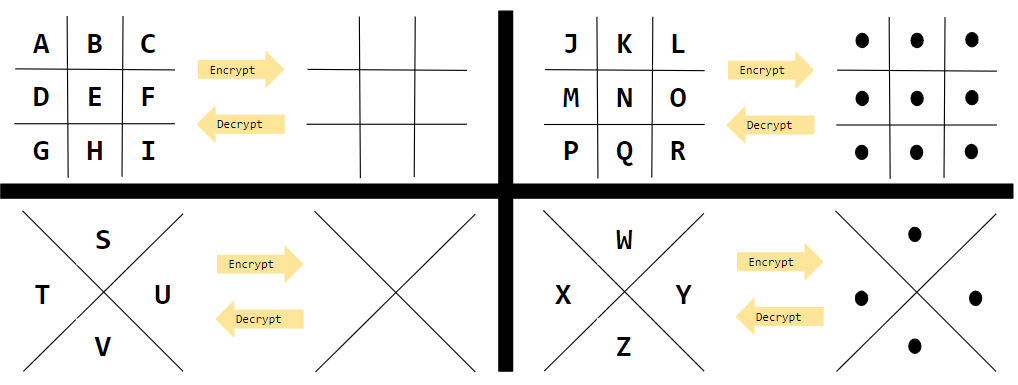
\includegraphics[scale=0.75]{assets/masonic_ex1.png}
\end{center}
The idea is that we can replace a letter (e.g., \code{A}) with a corresponding geometric shape (e.g., the backwards \code{L} represented by the top-left part of the grid.) 

\bigskip 

Some other examples based on the above cipher are shown below:
\begin{center}
    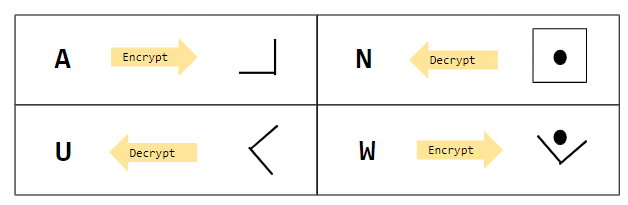
\includegraphics[scale=0.9]{assets/masonic_ex2.png}
\end{center}
Note that there is \emph{no key} associated with this cipher. There is only a decryption function (which is just mapping the geometric shape back to the letter). Therefore, the adversary, who knows that a message was encrypted using a masonic cipher, can recover the plaintext easily. 


\subsection{Caesar Cipher}
The Caesar cipher, also known as a \emph{shift cipher}, is a simple substitution cipher that \emph{shifts} a letter by some amount $n$. Hence, the key for this cipher is an integer $n$. The idea is that we initially assign each letter an integer, perhaps by their alphabetical ranking (e.g., $A$ is 0, $B$ is 1, and so on.) If we want to shift the letters by some number, we can just ``move'' the letters by that amount. If a letter gets a new integer that's greater than 25, we can ``wrap'' the letter back.  

\bigskip 

Consider the following diagram, which shows the correspondence between the plaintext alphabet and the ciphertext alphabet.
\begin{center}
    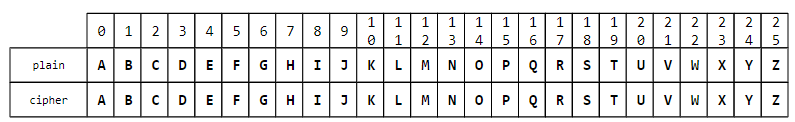
\includegraphics[scale=0.75]{assets/ceasar_1.png}
\end{center}
In this particular diagram, when we apply a shift, we apply the shift to the \emph{plain} row. By doing this, we can translate whatever plaintext we have to ciphertext. 

\begin{mdframed}
    (Example.) If we shift each letter by 3 (i.e., $n = 3$), we have 
    \begin{center}
        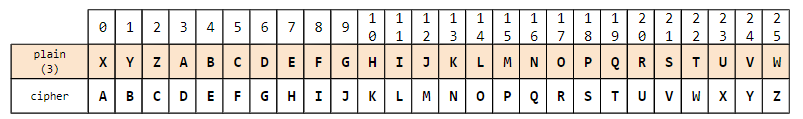
\includegraphics[scale=0.7]{assets/ceasar_2.png}
    \end{center}
    Notice how $A$ now corresponds to 3. Recall that $A$'s original position was 0; if we shift each letter by 3, we essentially add 3 to $A$'s original position to get the new position 
    \[0 + 3 = 3.\]
    The same idea applies to any other letter. One key thing to notice is how $X$, $Y$, and $Z$ were \emph{wrapped back} to the beginning. In any case, let's see how translation would work in this case: 
    \begin{itemize}
        \item To convert a letter from plaintext to ciphertext, look for the letter in the(shifted) plaintext row and then look at the corresponding ciphertext column. For example, $R$ in plaintext would become $U$ in ciphertext. 
        \item To convert a letter from ciphertext to plaintext, look for the letter in the ciphertext row and then look at the corresponding (shifted) plaintext column. For example, $U$ in ciphertext becomes $R$ in plaintext. 
    \end{itemize}
\end{mdframed}

\begin{mdframed}
    (Example.) If we shift each letter by -2 (i.e., $n = -2$), we have 
    \begin{center}
        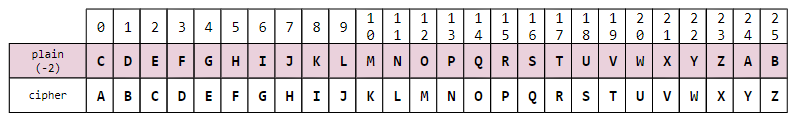
\includegraphics[scale=0.7]{assets/ceasar_3.png}
    \end{center}
\end{mdframed}

As with rectangular tranposition, we should encode the message by removing any non-alphabetic characters and capitalizing everything. 

\begin{mdframed}
    (Exercise.) 
    \begin{itemize}
        \item \emph{Using a shift of 3, encrypt the message \code{Meet at La Jolla Shores.}}
        \begin{mdframed}
            Encoding the message gives us \code{MEETATLAJOLLASHORES}. Then, we can use the example above (with the shift of 3) to give us the proper correspondence.
            \begin{verbatim}
    plain       M E E T A T L A J O L L A S H O R E S
    cipher      P H H W D W O D M R O O D V K R U H V\end{verbatim}
            This gives us \code{PHHWDWODMROODVKRUHV}.
        \end{mdframed}
        \item \emph{Using a shift of 3, decrypt the message \code{PHHWDWVXQJRGODZQ}}
        \begin{mdframed}
            Using the example above (with the shift of 3), we have
            \begin{verbatim}
    cipher      P H H W D W V X Q J R G O D Z Q
    plain       M E E T A T S U N G O D L A W N\end{verbatim}
            Decoding this gives us \code{Meet at Sun God Lawn.}
        \end{mdframed}
    \end{itemize}
\end{mdframed}

\begin{mdframed}
    (Exercise.) \emph{You are Eve. You have just intercepted the following message that Alice was trying to send to Bob: \code{Q TQDM IB QPWCAM}. You know that Alice used a Caesar cipher, but she didn't remove spaces before encrypting: she left the spaces in her original message as-is. What is the original message?}
    
    \begin{mdframed}
        \code{Q} itself could be a word; specifically, it could either be \code{A} or \code{I}. We can try to figure out what the message by guessing which word the first word could be. 
        \begin{itemize}
            \item If \code{Q} maps to \code{A}, then we have 
            \begin{center}
                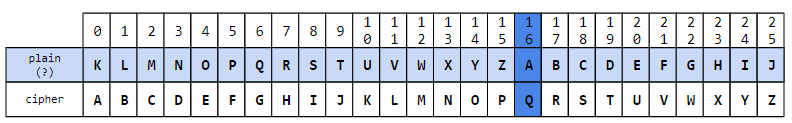
\includegraphics[scale=0.6]{assets/ceasar_4.png}
            \end{center}
            Partially decrypting the ciphertext gives us \code{A DANW}, but \code{DANW} is meaningless. Therefore, it cannot be \code{A}. 

            \item If \code{Q} maps to \code{I}, then we have
            \begin{center}
                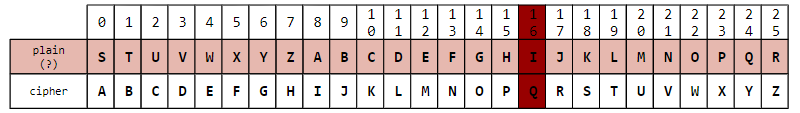
\includegraphics[scale=0.6]{assets/ceasar_5.png}
            \end{center}
            Decrypting this gives us: 
            \begin{verbatim}
                I LIVE AT IHOUSE\end{verbatim}
        \end{itemize}
        Therefore, the message is \code{I LIVE AT IHOUSE}. The shift was 8.
    \end{mdframed}
\end{mdframed}


\begin{mdframed}
    (Exercise.) Alice encrypts the following message using a Caesar cipher with a shift of 1. 
    \begin{verbatim}
Zeus is hiding in a cave \end{verbatim}
    What is the corresponding ciphertext? 
    \begin{mdframed}
        \begin{verbatim}
plain       ZEUSISHIDINGINACAVE
cipher      AFVTJTIJEJOHJOBDBWF\end{verbatim}
        Essentially, we just move all letters forward by 1.
    \end{mdframed}
\end{mdframed}


\subsection{Interlude: Modular Arithmetic}
One fundamental idea in number theory, which is used in cryptography, is modular arithmetic. 

\subsubsection{Quotients and Remainders}

\begin{lemma}{Euclid's Division}{}
    For any integer $a$ and positive integer $n$, there exists a unique pair of integers $q$ and $r$ such that $0 \leq r < n$ and $a = qn + r$. The integers $q$ and $r$ are called the quotient and remainder, respectively. We also write $a \Mod{n}$ to refer to the remainder.
\end{lemma}
For the proof, the deal is that we can keep subtracting, or adding, $n$ from $a$ until we end up in the range $[0, n)$. Therefore, the number of times we had to subtract, or add, $n$ is the \emph{quotient}, and the number in the range $[0, n)$ that we end up with at the end is the \emph{remainder}. 

\begin{mdframed}
    (Example.) Divide $a = 17$ by $n = 5$. Find the quotient and remainder.
    
    \bigskip 

    Using the proof idea, we note that: 
    \begin{itemize}
        \item Subtracting 5 to $a$ once gives us 12. 
        \item Subtracting 5 to $a$ twice gives us 7.
        \item Subtracting 5 to $a$ thrice gives us 2.
    \end{itemize}
    It took us 3 subtractions to get to a number that's in the range $[0, 5)$, so the quotient is $\boxed{3}$ and the remainder is $\boxed{2}$. 
\end{mdframed}
We should note that this is pretty standard when $a \geq 0$. However, for $a < 0$, it might be less familiar, albeit the same process.

\begin{mdframed}
    (Example.) Divide $a = -7$ by $n = 5$. Find the quotient and remainder.

    \bigskip 

    Using the proof idea, we note that: 
    \begin{itemize}
        \item Adding 5 to $a$ once gives us 2.
        \item Adding 5 to $a$ twice gives us 3. 
    \end{itemize}
    It took us 2 additions to get to a number that's in the range $[0, 5)$, so the quotient is $\boxed{-2}$ (because we had to \emph{add}, not subtract) and the remainder is $\boxed{3}$. 
\end{mdframed}

\textbf{Remark:} 
\begin{itemize}
    \item If we have to \textbf{add} $n$ to $a$ $x$ times to get a number that's in the range $[0, n)$, then our final quotient will be negative (that is, $-x$).
    \item If we have to \textbf{subtract} $n$ from $a$ $x$ times to get a number that's in the range $[0, n)$, then our final quotient will be positive (that is, $x$).
\end{itemize}

\begin{mdframed}
    (Exercise.) For each of the following, calculate the quotient and remainder when $a$ is divided by $n$. Do these calculations by hand. 
    \begin{itemize}
        \item $a = 13$, $n = 3$.
        \begin{mdframed}
            We know that $13 / 3 = 4$, and $13 - (3 \cdot 4) = 1 \in [0, 3)$. So, the quotient is \boxed{4} and the remainder is \boxed{1}. 
        \end{mdframed}
        \item $a = 134$, $n = 10$.
        \begin{mdframed}
            We know that $134 / 10 = 13$ and $134 - (10 \cdot 13) = 4 \in [0, 10)$. So, the quotient is \boxed{13} and remainder is \boxed{4}.
        \end{mdframed}
        \item $a = -37$, $n = 10$.
        \begin{mdframed}
            We know that we need to add $n$ to $a$ \textbf{4} times to get a number, $3$, that is in the range $[0, 10)$. To be precise, 
            \[-37 + 10 + 10 + 10 + 10 = -37 + 40 = 3 \in [0, 10).\]
            Therefore, the quotient is \boxed{-4} and the remainder is \boxed{3}. 
        \end{mdframed}
        \item $a = -15$, $n = 60$.
        \begin{mdframed}
            We have to add $n$ to $a$ \textbf{1} time to get $45 \in [0, 60)$. Therefore, the quotient is \boxed{-1} and the remainder is \boxed{45}.
        \end{mdframed}
        \item $a = 13$, $n = 12$.
        \begin{mdframed}
            We know that $13 / 12 = 1$ and $13 - (12 \cdot 1) = 1$. So, the quotient is \boxed{1} and the remainder is \boxed{1}.
        \end{mdframed}
    \end{itemize}
\end{mdframed}

\begin{mdframed}
    (Exercise.) What is $-13 \Mod{5}$?
    \begin{mdframed}
        \[-13 + 5 + 5 + 5 = 2 \in [0, 5),\]
        so the quotient is $-3$ (since we had to perform 3 additions) and the remainder is \boxed{2}. Therefore, 
        \[-13 \Mod{5} = 2.\]
    \end{mdframed}
\end{mdframed}

\begin{proposition}
    Suppose $a$ and $n$ are integers and $n > 0$. All the following statements are equivalent:
    \begin{itemize}
        \item $a \Mod{n} = 0$.
        \item There is no remainder when $a$ is divided by $n$. 
        \item $a$ is a multiple of $n$. 
        \item $a$ is divisible by $n$. 
        \item $n$ is a divisor of $a$. 
        \item $n$ is a factor of $a$. 
        \item $n$ divides $a$ (in notation\footnote{Note that $\vert$ is read as ``\emph{divides}.''}: $n \vert a$).
        \item $a / n$ is an integer.
    \end{itemize}
\end{proposition}

\subsubsection{Congruences}
\begin{definition}{Congruence}{}
    Fix a positive integer $n$. If $a$ and $b$ are integers, we say that ``$a$ is \textbf{congruent} to $b$ mod $n$,'' or that ``$a$ and $b$ are congruent mod $n$,'' if $a$ and $b$ have the same remainder when each is divided by $n$. This can be denoted in symbols as follows: 
    \[a \equiv b \Mod{n}.\] 
\end{definition}
For example, $19 \equiv 7 \Mod{4}$ since $19$ and $7$ both have remainder 3 when divided by 4. Observe also that $19 - 7 = 12$ is a multiple of 4. This can be generalized: 

\begin{lemma}{}{}
    Fix a positive integer $n$. Two integers $a$ and $b$ are congruent mod $n$ if and only if $a - b$ is a multiple of $n$.
\end{lemma}

\begin{proof}
    Divide $a$ and $b$ by $n$ to write $a = q_1 n + r_1$ and $b = q_2 n + r_2$. If \[a \equiv b \Mod{n},\] this by definition means that $r_1 = r_2$ so 
    \[a - b = (q_1 n + r_1) - (q_2 n + r_2) = q_1 n - q_2 n = n(q_1 - q_2).\]
    So, $a - b$ is a multiple of $n$. Conversely, suppose $a - b$ is a multiple of $n$. Then, 
    \[(a - b) - (q_1 - q_2)n = ((q_1 n + r_1) - (q_2 n + r_2)) - (q_1 - q_2)n = r_1 - r_2\]
    is a multiple of $n$. Since $0 \leq r_1, r_2 < n$, however, we must have $|r_1 - r_2| < n$. The only way that $r_1 - r_2$ can be a multiple of $n$ is if $r_1 - r_2 = 0$, i.e., if $r_1 = r_2$. That means $a \equiv b \Mod{n}$. 
\end{proof}

\begin{theorem}{Modular Arithmetic Theorem}{}
    Fix a positive integer $n$. Suppose $a$, $a'$, $b$, $b'$ are integers such that 
    \[a \equiv a' \Mod{n}\]
    \[b \equiv b' \Mod{n}\]
    and $k$ is any positive integer. Then, all of the following are also true: 
    \[a + b \equiv a' + b' \Mod{n}\]
    \[a - b \equiv a' - b' \Mod{n}\]
    \[ab \equiv a'b' \Mod{n}\]
    \[a^k \equiv (a')^k \Mod{n}\]
\end{theorem}

\begin{mdframed}
    (Exercise.) Use the Modular Arithmetic Theorem to quickly calculate the following. 
    \begin{itemize}
        \item $417 \cdot 22 \Mod{10}$.
        \begin{mdframed}
            \begin{equation*}
                \begin{aligned}
                    417 \cdot 22 &\equiv 7 \cdot 2  \\ 
                        &= 14 \\ 
                        &\equiv 4 \Mod{10}.
                \end{aligned}
            \end{equation*}
        \end{mdframed}
        \item $333333 + 666 \Mod{3}$.
        \begin{mdframed}
            \begin{equation*}
                \begin{aligned}
                    333333 + 666 &\equiv 0 + 0 \\ 
                        &\equiv 0 \Mod{3}.
                \end{aligned}
            \end{equation*}
        \end{mdframed}
        \item $7^{202320232023} \Mod{6}$. 
        \begin{mdframed}
            \begin{equation*}
                \begin{aligned}
                    7^{202320232023} &= 7 \cdot 7 \cdot \hdots \cdot 7 \\ 
                        &\equiv 1 \cdot 1 \cdot \hdots \cdot 1 \\ 
                        &= 1 \Mod{6}.
                \end{aligned}
            \end{equation*}
        \end{mdframed}
        \item What is $5^{2023202320232023} \Mod{6}$?
        \begin{mdframed}
            \begin{equation*}
                \begin{aligned}
                    5^{2023202320232023} &= 5 \cdot 5 \cdot \hdots \cdot 5 \\ 
                        &\equiv (-1) \cdot (-1) \cdot \hdots \cdot (-1) \\ 
                        &= (-1)^{2023202320232023} \\ 
                        &\equiv -1 \\ 
                        &\equiv 5 \Mod{6}.
                \end{aligned}
            \end{equation*}
            Therefore, the answer is \boxed{5}.
        \end{mdframed}
    \end{itemize}
\end{mdframed}

\begin{mdframed}
    (Exercise.) Fix positive integers $k$ and $n$. Suppose $a$ and $a'$ are integers such that $a \equiv a' \Mod{n}$. It is not true in general that $k^a \equiv k^{a'} \Mod{n}$. Show this by example: in other words, find $k$, $n$, $a$, and $a'$ such that $a \equiv a' \Mod{n}$ but $k^a \not\equiv k^{a'} \Mod{n}$. 

    \begin{mdframed}
        Let $k = 2$, $n = 5$, $a = 6$, and $a' = 1$ so that 
        \[6 \equiv 1 \Mod{5}.\]
        Then, we note that 
        \[k^a = 2^6 = 64\]
        and 
        \[k^{a'} = 2^1 = 2.\]
        From this, it's clear that 
        \[64 \not\equiv 2 \Mod{5}.\]
    \end{mdframed}
\end{mdframed}

\begin{mdframed}[nobreak=true]
    (Exercise.) \emph{Suppose that the number $273x49y5$, where $x$ and $y$ are unknown digits, is divisible by 495. Find $x$ and $y$.}
    \begin{mdframed}
        We are asked to solve 
        \[273x49y5 \equiv 0 \mod{495}.\]

        We can write $273x49y5$ as 
        \[20000000 + 7000000 + 300000 + 10000x + 4000 + 900 + 10000y + 5.\]
        With this in mind, we have
        \begin{equation*}
            \begin{aligned}
                20000000 &+ 7000000 + 300000 + 10000x + 4000 + 900 + 10y + 5 \\ 
                    &\equiv 20 + 205 + 30 + 100x + 40 + 405 + 10y + 5 \\ 
                    &= 705 + 100x + 10y \\ 
                    &\equiv 210 + 100x + 10y \mod{495}.
            \end{aligned}
        \end{equation*}
        We note that the next multiple of 495 is 990. So, effectively, we want to find some $x$ and $y$ such that $0 \leq x < 10$ and $0 \leq y < 10$ and
        \[210 + 100x + 10y = 990.\]
        This gives us 
        \[100x + 10y = 780.\]
        One obvious solution is $x = 7$ and $y = 8$. 
    \end{mdframed}
\end{mdframed}


\subsubsection{Revisiting the Caesar Cipher}
Suppose we identify the letters $A$ through $Z$ with the numbers 0 through 25. In other words, we have $A \mapsto 0$, $B \mapsto 1$, and so on. Suppose we want to apply the Caesar cipher with a shift of 5 to encrypt the letter $Y$. Consider the following 
\[E(x) = (x + 5) \Mod{26}.\]
We note that $Y$ corresponds to the number 24. Then, it follows that 
\[E(24) = (24 + 5) \Mod{26} = 29 \Mod{26} = 3.\]
The number 3 corresponds to the letter $D$, the desired result. In other words, if we can identify the letters with numbers, the function $E$ is the encryption function of the Caesar cipher with a shift of 5.  

\bigskip 

The decryption function is given by 
\[D(y) = (y - 5) \Mod{26}.\]
So, if we wanted to decrypt the letter $D$, which corresponds to the number 3, then 
\[D(3) = (3 - 5) \Mod{26} = -2 \Mod{26} = 24,\]
which corresponds to $Y$. 

\bigskip 

What we just did is actually a consequence of the Modular Arithmetic Theorem; for a quick little ``proof,'' notice how  
\begin{equation*}
    \begin{aligned}
        D(E(x)) &= D(y) \\
            &\equiv (y - 5) \Mod{26} \\ 
            &\equiv ((x + 5) - 5) \Mod{26} \\ 
            &= x.
    \end{aligned} 
\end{equation*}

\begin{mdframed}
    (Exercise.) Decipher the message below, which was encrypted using a Caesar cipher with a shift of 3 and then using a rectangular transposition with the keyword \code{EARLY}.
    \begin{verbatim}
        DKSSBUIGLDEBXOX\end{verbatim}

    \begin{mdframed}
        To decrypt this message, we need to work backwards: first, use rectangular transposition to undo the first encryption, and then Caesar cipher to undo the second encryption.
        \begin{enumerate}
            \item For the rectangular transposition, note that the keyword has alphabetical ranking \code{21435}, so using the streamlined way discussed earlier, we have 
            \begin{mdframed}
                \begin{verbatim}
12345    21435
DKSSB -> KDSSB
UIGLD -> IULGD
EBXOX -> BEOXX\end{verbatim}
            \end{mdframed}
            Unstacking gives us \code{KDSSBIULGDBEOXX}.

            \item Next, we need to undo the Caesar cipher encryption on the message that we found from the previous step. Since the encryption used a positive shift of 3, undoing it requires us to use a negative shift of 3. This gives us: 
            \begin{mdframed}
                \begin{verbatim}
encrypted   KDSSBIULGDBEOXX
decrypted   HAPPYFRIDAY....\end{verbatim}
            \end{mdframed}
            Note that the last four letters were omitted. In any case, this gives us the decoded message \code{Happy Friday}.
        \end{enumerate}
    \end{mdframed}
\end{mdframed}
\textbf{Remark:} You should not assume that these operations are commutative. That is, if we were to decrypt the message by applying the Caesar cipher first and then the rectangular transposition, as opposed to the reverse order, we may get a different answer!


\subsection{Interlude: GCDs}
\begin{definition}{Greatest Common Divisor}{}
    The \textbf{greatest common divisor} (or \emph{GCD}) of two integers $a$ and $b$ that are not both zero is denoted $\gcd(a, b)$ and is defined to be the largest integer which is both a divisor of $a$ and a divisor of $b$.
\end{definition}

\begin{mdframed}
    (Example.) Suppose we wanted to compute $\gcd(14, 21)$. 
    \begin{itemize}
        \item The factors of 14 are 1, 2, 7, and 14.
        \item The factors of 21 are 1, 3, 7, and 21. 
    \end{itemize}
    Therefore, as 7 is the \emph{largest integer} which is both a divisor of 14 and 21, it follows that $\gcd(14, 21) = 7$.
\end{mdframed}
Note that, while intuitive, this is actually not the best way of finding GCDs. Finding the factors of a number, especially a large one, is difficult. However, there exists algorithms that we can use to quickly calculate GCDs.

\begin{mdframed}
    (Example.) Suppose $a$ is a nonzero integer. What is $\gcd(a, 0)$?

    \begin{mdframed}
        The answer is $\gcd(a, 0) = |a|$. To see why this is the case, consider the following points. 

        \begin{enumerate}
            \item If $a \neq 0$, the largest value that divides $a$ is $|a|$. 
            \begin{mdframed}
                For example, the largest value that divides $100$ is $|100| = 100$. Likewise, the largest value that divides $-100$ is still $|-100| = 100$. 
            \end{mdframed}

            \item If you think about it, all integers divide 0. 
            \begin{mdframed}
                Recall that, if $a$ and $b$ are integers, $a$ divides $b$ if there is an integer $c$ such that 
                \[ac = b.\]
                Here, we write that $a | b$ to mean that $a$ divides $b$. 

                \bigskip 

                With this in mind, we note that 
                \[a \cdot 0 = 0\]
                and therefore 
                \[a | 0.\]
            \end{mdframed}

            \item Therefore, it follows that $\gcd(a, 0) = |a|$. 
            \begin{mdframed}
                To see this, note that the factors of $10$ and $-10$ are 
                \[\{-10, -5, -2, -1, 1, 2, 5, 10\},\]
                and we know that all factors of $0$ are effectively all integers. Therefore, it follows that 10 would be the answer here. 
            \end{mdframed}
        \end{enumerate}
    \end{mdframed}
\end{mdframed}

\subsubsection{Euclidean Algorithm}
The Euclidean Algorithm for computing GCDs relies on the following observation, defined as a lemma. 
\begin{lemma}{}{}
    Let $n$ be a positive integer and $a \equiv b \Mod{n}$. Then, $\gcd(a, n) = \gcd(b, n)$. 
\end{lemma}

\begin{proof}
    Let $c = \gcd(a, n)$ and $d = \gcd(b, n)$. Let $k$ be an integer such that \[a - b = nk.\] Since $c$ is a factor of both $a$ and $n$, it is also a factor of $a - nk = b$. Thus, $c$ is a common factor of both $b$ and $n$ as well, so $c \leq d$ bby definition of $d$. On the other hand, the same logic shows that $d$ is a common factor of both $a$ and $n$, so $d \leq c$ and thus $d = c$. 
\end{proof}

\begin{corollary}{}{}
    Let $n$ be a positive integer and let $r$ be the remainder when an integer $a$ is divided by $n$. Then, $\gcd(a, n) = \gcd(r, n)$. 
\end{corollary}

This brings us to the Euclidean Algorithm: 
\begin{mdframed}
    Suppose $a$ and $b$ are two positive integers, and assume without loss of generality (WLOG) that $b \geq a$. To find $\gcd(a, b)$, we can do the following: 
    \begin{itemize}
        \item Divide $b$ by $a$ and let $r$ be the remainder. Then, 
        \begin{itemize}
            \item If $r = 0$, output $a$. 
            \item Otherwise, replace $b$ with $a$ and $a$ with $r$. Then, repeat. 
        \end{itemize}
    \end{itemize}
\end{mdframed}

\begin{mdframed}
    (Example.) Suppose we wanted to compute $\gcd(115, 35)$. We divide the bigger number by the smaller one and get 
    \[115 = 3 \cdot 35 + 10.\]
    The remainder, $r = 10$, is nonzero, so we'll divide again, but this time, we'll divide the dividend (35) by the remainder (10) to get 
    \[35 = 3 \cdot 10 + 5.\]
    The remainder is nonzero again, so we repeat to get 
    \[10 = 2 \cdot 5 + 0.\]
    Since the remainder is 0, we output the dividend: \boxed{5}. Therefore, 
    \[\gcd(115, 35) = 5.\]
\end{mdframed}

\begin{mdframed}
    (Exercise.) Compute the following GCDs using the Euclidean Algorithm.

    \begin{itemize}
        \item $\gcd(180, 120).$
        \begin{mdframed}
            \begin{center}
                \begin{tabular}{|c|c|c|c|c|}
                    \hline 
                    $\mathbf{a}$ & $\mathbf{b}$ & $\mathbf{b = aq + r}$ & $\mathbf{q}$ & $\mathbf{r}$ \\ 
                    \hline 
                    120 & 180 & $180 = 120q + r$ & 1   & 60 \\ 
                    60  & 120 & $120 = 60q + r$  & 2   & 0  \\ 
                    \hline 
                \end{tabular}
            \end{center}
            Therefore, the answer must be \boxed{60}.
        \end{mdframed}
        \item $\gcd(180, 81).$
        \begin{mdframed}
            \begin{center}
                \begin{tabular}{|c|c|c|c|c|}
                    \hline 
                    $\mathbf{a}$ & $\mathbf{b}$ & $\mathbf{b = aq + r}$ & $\mathbf{q}$ & $\mathbf{r}$ \\ 
                    \hline 
                    81 & 180 & $180 = 81q + r$ & 2 & 18 \\ 
                    18 & 81 & $81 = 18q + r$ & 4 & 9 \\ 
                    9 & 18 & $18 = 9q + r$ & 2 & 0 \\ 
                    \hline 
                \end{tabular}
            \end{center}
            Therefore, the answer must be \boxed{9}.
        \end{mdframed}
        \item $\gcd(121, 77).$
        \begin{mdframed}
            \begin{center}
                \begin{tabular}{|c|c|c|c|c|}
                    \hline 
                    $\mathbf{a}$ & $\mathbf{b}$ & $\mathbf{b = aq + r}$ & $\mathbf{q}$ & $\mathbf{r}$ \\ 
                    \hline 
                    77 & 121 & $121 = 77q + r$ & 1 & 44 \\ 
                    44 & 77 & $77 = 44q + r$ & 1 & 33 \\ 
                    33 & 44 & $44 = 33q + r$ & 1 & 11 \\ 
                    11 & 33 & $33 = 11q + r$ & 3 & 0 \\ 
                    \hline 
                \end{tabular}
            \end{center}
            Therefore, the answer must be \boxed{11}.
        \end{mdframed}
    \end{itemize}
\end{mdframed}

\subsubsection{Bezout's Theorem}
\begin{theorem}{Bezout's Theorem}{}
    Suppose $a$ and $b$ are integers not both 0. Then, $\gcd(a, b)$ can be written as an \emph{integer linear combination} of $a$ and $b$, i.e., it can be written as $ax + by$ for some integers $x$ and $y$. Integers $x$ and $y$ such that \[\gcd(a, b) = ax + by\] are called \textbf{Bezout's coefficients}.
\end{theorem}

We can use the Euclidean Algorithm to find the Bezout coefficients, as seen in the example below. 
\begin{mdframed}
    (Example.) Suppose we want to find the Bezout coefficients for $\gcd(115, 35)$. Recall the sequence of operations we had to do:
    \[115 = 3 \cdot 35 + 10.\]
    \[35 = 3 \cdot 10 + 5.\]
    \[10 = 2 \cdot 5 + 0.\]
    Suppose we rearrange the first and second equations, like so: 
    \[10 = 115 - 3 \cdot 35.\] 
    \[5 = 35 - 3 \cdot 10.\]
    Plugging in the first equation into the second equation gives us 
    \[5 = 35 - 3 \cdot (115 - 3 \cdot 35).\]
    Simplifying this gives us 
    \begin{equation*}
        \begin{aligned}
            5 &= 35 - 3 \cdot (115 - 3 \cdot 35) \\ 
                &= 35 - 3(115) + 9(35) \\ 
                &= 10(35) - 3(115).
        \end{aligned}
    \end{equation*}
    Notice how we wrote $\gcd(115, 35)$ as an integer linear combination of those two numbers.
\end{mdframed}

Essentially, the steps are as follows: 
\begin{enumerate}
    \item Find the GCD using the Euclidean Algorithm.
    \item Rewrite the division for the \emph{last nonzero remainder}. 
    \item Alternate between substitution for the remainder directly above, and then simplify. Alternatively, start from the last equation with a nonzero remainder and then keep using the equations before that equation (e.g., from equation $n$, the last equation with a nonzero remainder, substitute equation $n - 1$ in the next step. Then, in the next step, substitute equation $n - 2$. Keep doing this until you reach equation 1.)
\end{enumerate}

\begin{mdframed}
    (Example.) Suppose we want to find the Bezout coefficients for $\gcd(240, 46)$. 
    \begin{enumerate}
        \item First, let's compute the GCD, keeping note of the sequence of operations we made. 
        \begin{center}
            \begin{tabular}{|c|c|c|c|c|}
                \hline 
                $\mathbf{a}$ & $\mathbf{b}$ & $\mathbf{b = aq + r}$ & $\mathbf{q}$ & $\mathbf{r}$ \\ 
                \hline 
                46 & 240 & $240 = 46q + r$ & 5 & 10 \\ 
                10 & 46 & $46 = 10q + r$ & 4 & 6 \\ 
                6 & 10 & $10 = 6q + r$ & 1 & 4 \\ 
                4 & 6 & $6 = 4q + r$ & 1 & 2 \\ 
                2 & 4 & $4 = 2q + r$ & 2 & 0 \\
                \hline 
            \end{tabular}
        \end{center}
        This tells us that $\gcd(240, 46) = 2$. The operations we did were 
        \begin{itemize}
            \item (Eq. 1) $240 = 46(5) + 10 \implies 10 = 240 - 46 \cdot 5$
            \item (Eq. 2) $46 = 10(4) + 6 \implies 6 = 46 - 10 \cdot 4$
            \item (Eq. 3) $10 = 6(1) + 4 \implies 4 = 10 - 6 \cdot 1$
            \item (Eq. 4) $6 = 4(1) + 2 \implies 2 = 6 - 4 \cdot 1$
            \item (Eq. 5) $4 = 2(2) + 0$
        \end{itemize}

        \item Rewriting the division for the last equation with the nonzero remainder (Eq. 4) gives us $2 = 6 - 4 \cdot 1.$
        \item Starting from the division for the last nonzero remainder, let's rewrite it: 
        \begin{equation*}
            \begin{aligned}
                2 &= 6 - 4 \cdot 1 && \text{From Eq. 4} \\ 
                    &= 6 - (\underbrace{10 - 6 \cdot 1}_{\text{Eq. 3}}) \cdot 1 && \text{Substitute Eq. 3} \\ 
                    &= 6 - 10 + 6 && \text{Expand} \\ 
                    &= 2 \cdot 6 - 1 \cdot 10 && \text{Rewrite to group like terms} \\ 
                    &= 2 \cdot (\underbrace{46 - 10 \cdot 4}_{\text{Eq. 2}}) - 1 \cdot 10 && \text{Substitute Eq. 2} \\ 
                    &= 2 \cdot 46 - 2 \cdot 10 \cdot 4 - 1 \cdot 10 && \text{Expand} \\ 
                    &= 2 \cdot 46 - 8 \cdot 10 - 1 \cdot 10 && \text{Simplify} \\ 
                    &= 2 \cdot 46 - 9 \cdot 10 && \text{Rewrite to group like terms} \\ 
                    &= 2 \cdot 46 - 9 \cdot (\underbrace{240 - 46 \cdot 5}_{\text{Eq. 1}}) && \text{Substitute Eq. 1} \\ 
                    &= 2 \cdot 46 - 9 \cdot 240 + 46 \cdot 5 \cdot 9 && \text{Expand} \\ 
                    &= 2 \cdot 46 - 9 \cdot 240 + 46 \cdot 45 && \text{Simplify} \\ 
                    &= 47 \cdot 46 - 9 \cdot 240 && \text{Rewrite to group like terms}
            \end{aligned}
        \end{equation*}
        Notice how the Bezout coefficients are $47$ and $-9$. 
    \end{enumerate}
\end{mdframed}

\begin{mdframed}
    (Exercise.) Calculate Bezout's coefficients for the following GCDs using the extended Euclidean Algorithm.
    \begin{itemize}
        \item $\gcd(180, 120).$
        \begin{mdframed}
            \begin{enumerate}
                \item First, compute the GCD. We already did this in a previous exercise, but just to reiterate: 
                \begin{center}
                    \begin{tabular}{|c|c|c|c|c|}
                        \hline 
                        $\mathbf{a}$ & $\mathbf{b}$ & $\mathbf{b = aq + r}$ & $\mathbf{q}$ & $\mathbf{r}$ \\ 
                        \hline 
                        120 & 180 & $180 = 120q + r$ & 1   & 60 \\ 
                        60  & 120 & $120 = 60q + r$  & 2   & 0  \\ 
                        \hline 
                    \end{tabular}
                \end{center}
                Therefore, the GCD is 60. The operations that we did were 
                \begin{itemize}
                    \item (Eq. 1) $180 = 120(1) + 60 \implies 60 = 180 - 120(1)$
                    \item (Eq. 2) $120 = 60(2) + 0$
                \end{itemize}


                \item Next, we just need to rewrite the last equation with a nonzero remainder. 
                \[180 = 120(1) + 60 \implies 60 = 180 - 120(1)\]

                \item Finally, we need to work backwards, substituting the previous equations. Because we only have one operation which resulted in a non-zero remainder, it follows that we only need to do: 
                \[60 = 180 - 120(1).\]
                Therefore, the Bezout coefficients are \boxed{1} and \boxed{-1}.
            \end{enumerate}
        \end{mdframed}
        \item $\gcd(180, 81).$
        \begin{mdframed}
            \begin{enumerate}
                \item First, we need to compute the GCD. We already did this in a previous exercise, but to reiterate: 
                
                \begin{center}
                    \begin{tabular}{|c|c|c|c|c|}
                        \hline 
                        $\mathbf{a}$ & $\mathbf{b}$ & $\mathbf{b = aq + r}$ & $\mathbf{q}$ & $\mathbf{r}$ \\ 
                        \hline 
                        81 & 180 & $180 = 81q + r$ & 2 & 18 \\ 
                        18 & 81 & $81 = 18q + r$ & 4 & 9 \\ 
                        9 & 18 & $18 = 9q + r$ & 2 & 0 \\ 
                        \hline 
                    \end{tabular}
                \end{center}
                Therefore, the GCD is 9. The operations we did were 
                \begin{itemize}
                    \item (Eq. 1) $180 = 81(2) + 18 \implies 18 = 180 - 81(2)$
                    \item (Eq. 2) $81 = 18(4) + 9 \implies 9 = 81 - 18(4)$ 
                    \item (Eq. 3) $18 = 9(2) + 0$
                \end{itemize}
        


                \item Next, we need to rewrite the last equation with a nonzero remainder. 
                \[81 = 18(4) + 9 \implies 9 = 81 - 18(4).\]

                \item Finally, we need to work backwards, substituting the previous equations as needed. 
                \begin{equation*}
                    \begin{aligned}
                        9 &= 81 - 18(4) \\ 
                            &= 81 - (\underbrace{180 - 81(2)}_{\text{Eq. 1}}) \cdot 4 \\ 
                            &= 81 - 180(4) + 81(8) \\ 
                            &= 81(9) - 180(4) 
                    \end{aligned}
                \end{equation*}

                Therefore, the Bezout coefficients are \boxed{9} and \boxed{-4}.
            \end{enumerate}



        \end{mdframed}
        \item $\gcd(121, 77).$
        \begin{mdframed}
            \begin{enumerate}
                \item First, compute the GCD. To reiterate:
                \begin{center}
                    \begin{tabular}{|c|c|c|c|c|}
                        \hline 
                        $\mathbf{a}$ & $\mathbf{b}$ & $\mathbf{b = aq + r}$ & $\mathbf{q}$ & $\mathbf{r}$ \\ 
                        \hline 
                        77 & 121 & $121 = 77q + r$ & 1 & 44 \\ 
                        44 & 77 & $77 = 44q + r$ & 1 & 33 \\ 
                        33 & 44 & $44 = 33q + r$ & 1 & 11 \\ 
                        11 & 33 & $33 = 11q + r$ & 3 & 0 \\ 
                        \hline 
                    \end{tabular}
                \end{center}
                Therefore, the GCD is 11. The operations that we did were 
                \begin{itemize}
                    \item (Eq. 1) $121 = 77(1) + 44 \implies 44 = 121 - 77(1)$ 
                    \item (Eq. 2) $77 = 44(1) + 33 \implies 33 = 77 - 44(1)$
                    \item (Eq. 3) $44 = 33(1) + 11 \implies 11 = 44 - 33(1)$
                    \item (Eq. 4) $33 = 11(3) + 0$
                \end{itemize}

                \item Next, rewrite the last equation with a nonzero remainder.
                \[44 = 33(1) + 11 \implies 11 = 44 - 33(1).\]

                \item Finally, work backwards. 
                \begin{equation*}
                    \begin{aligned}
                        11 &= 44 - 33(1) \\ 
                            &= 44 - (\underbrace{77 - 44(1)}_{\text{Eq. 2}}) \cdot 1 \\
                            &= 44 - 77 + 44(1) \\ 
                            &= 44(2) - 77 \\ 
                            &= (\underbrace{121 - 77(1)}_{\text{Eq. 1}}) \cdot 2 - 77 \\ 
                            &= 121(2) - 77(2) - 77 \\ 
                            &= 121(2) - 77(3).
                    \end{aligned}
                \end{equation*}
                Thereforem the Bezout coefficients are \boxed{2} and \boxed{-3}.
            \end{enumerate}
        \end{mdframed}
    \end{itemize}
\end{mdframed}

\begin{mdframed}
    (Exercise.) Observe that $\gcd(42, 12) = 6$. Show that the pairs $(-1, 4)$ and $(1, -3)$ are both Bezout coefficients for 42 and 12. 

    \begin{mdframed}
        \begin{itemize}
            \item For the pair $(-1, 4)$, we have 
            \[42(-1) + 12(4) = -42 + 48 = 6.\]

            \item For the pair $(1, -3)$, we have 
            \[42(1) + 12(-3) = 42 - 36 = 6.\]
        \end{itemize}
    \end{mdframed}
\end{mdframed}

\begin{mdframed}
    (Exercise.) Consider $\gcd(150, 90)$.
    
    \begin{enumerate}
        \item How many divisions do we need to do until we see a remainder of 0 when we use the Euclidean algorithm to compute $\gcd(150, 90)$?
        \begin{mdframed}
            \begin{center}
                \begin{tabular}{|c|c|c|c|c|}
                    \hline 
                    $\mathbf{a}$ & $\mathbf{b}$ & $\mathbf{b = aq + r}$ & $\mathbf{q}$ & $\mathbf{r}$ \\ 
                    \hline 
                    90 & 150 & $150 = 90q + r$ & 1 & 60 \\ 
                    60 & 90 & $90 = 60q + r$ & 1 & 30 \\ 
                    30 & 60 & $60 = 30q + r$ & 2 & 0 \\ 
                    \hline 
                \end{tabular}
            \end{center}
            We had to perform \textbf{3} divisions. 
        \end{mdframed}

        \item Find Bezout coefficients for $\gcd(150, 90)$. 
        \begin{mdframed}
            Noting that $\gcd(150, 90) = 30$ and the equations we worked with are 
            \begin{itemize}
                \item (Eq. 1) $150 = 90(1) + 60 \implies 60 = 150 - 90(1)$
                \item (Eq. 2) $90 = 60(1) + 30 \implies 30 = 90 - 60(1)$
                \item (Eq. 3) $60 = 30(2) + 0$
            \end{itemize}
            Starting with Eq. 2, we have 
            \begin{equation*}
                \begin{aligned}
                    30 &= 90 - 60(1) \\ 
                        &= 90 - (\underbrace{150 - 90(1)}_{\text{Eq. 1}})(1) \\ 
                        &= 90 - 150 + 90 \\ 
                        &= 90(2) + 150(-1).
                \end{aligned}
            \end{equation*}
            So, the Bezout coefficients are \boxed{2} and \boxed{-1}.
        \end{mdframed}
    \end{enumerate}
\end{mdframed}


\subsubsection{Modular Inversion}
Suppose you are asked to solve the equation 
\[5z = 7.\]
Intuitively, we can just divide both sides by 5. Stated differently, we can multiply both sides by $\frac{1}{5}$:
\[\left(\frac{1}{5}\right) \cdot 5z = \left(\frac{1}{5}\right) 7 \implies z = \frac{5}{7}.\]
In other words, we're able to ``cancel out'' the 5 that appears on the left-hand side, thus isolating $z$. 

\bigskip 

With modular inversion, we can recreate this process with \emph{congruences}. For example, suppose we want to solve 
\[5z \equiv 7 \Mod{11}.\]
We cannot ``divide both sides by 5'' because congruences only make sense when both sides of the congruence are \emph{integers}. But, if we find an integer $x$ with the property that 
\[5x \equiv 1 \Mod{11},\] 
then we can multiply both sides of our congruence by $x$ to effectively eliminate the 5 on the left-hand side. In this example, there \emph{is} an integer: $x = 9$. Using this integer, we have 
\[5x = 9 \cdot 5 = 45 \equiv 1 \Mod{11}.\]
Therefore, multiplying both sides of our congruence by 9 gives us 
\[z = 1 \cdot z \equiv (5 \cdot 9)z = 9 \cdot (5z) \equiv 9 \cdot 7 \Mod{11}.\]
Thus, 
\[z \equiv 9 \cdot 7 = 63 \equiv 8 \Mod{11},\]
and we've solved our congruence: $z \equiv 8 \Mod{11}$. While we solved this congruence, note that we basically guessed what the solution is. However, there's a way to get such $x$.

\begin{definition}{}{}
    Fix a positive integer $n$. An integer $a$ is \emph{invertible} mod $n$ (or a \emph{unit} mod $n$) if there exists another integer $x$ such that $ax \equiv 1 \Mod{n}$. The number $x$ is then called an \emph{inverse of} $a$ mod $n$ and, in symbols, one writes $x \equiv a^{-1} \Mod{n}$. 
\end{definition}
So, in the above example, we found that $9 \equiv 5^{-1} \Mod{11}$ because $5 \cdot 9 \equiv 1 \Mod{11}$. 

\begin{mdframed}
    (Exercise.) Explain why 2 is not invertible mod 4.
    \begin{mdframed}
        Essentially, we need to show why there does not exist an integer $x$ such that 
        \[2x \equiv 1 \Mod{4}.\]
        However, notice that both 2 and 4 are even. Therefore, multiplying 2 by any integer gives us an even number. Because 4 is even as well, it follows that we'll never be able to find an $x$ such that $2x \equiv 1 \Mod{4}$. 
    \end{mdframed}
\end{mdframed}

\begin{theorem}{Modular Inversion Theorem}{l3:1}
    Fix a positive integer $n$ and another integer $a$. Then, $a$ is invertible mod $n$ if and only if $\gcd(a, n) = 1$. Moreover, if $\gcd(a, n) = 1$ and $x$ and $y$ are Bezout coefficients for $a$ and $n$, then $x$ is an inverse of $a$ mod $n$. 
\end{theorem}

\begin{mdframed}
    (Example.) Suppose we want to find the inverse of $7 \Mod{23}$. Using the Euclidean Algorithm to compute $\gcd(23, 7)$, we get 
    \[23 = 3 \cdot 7 + 2\]
    \[7 = 3 \cdot 2 + 1\]
    \[2 = 2 \cdot 1 + 0.\]
    So, $\gcd(23, 7) = 1$ and thus 7 is in fact invertible mod 23. Working backwards, we find that 
    \begin{equation*}
        \begin{aligned}
            1 &= 7 - 3 \cdot 2 \\ 
                &= 7 - 3 \cdot (23 - 3 \cdot 7) \\ 
                &= 10 \cdot 7 - 3 \cdot 23.
        \end{aligned}
    \end{equation*}
    Therefore, the Modular Inversion Theorem tells us that 10 is the inverse of 7 mod 23. 
\end{mdframed}

\begin{mdframed}
    (Exercise.) Which of the following integers is invertible mod 210? 
    \begin{enumerate}[(a)]
        \item 3 
        \item 4
        \item 5
        \item None of the above 
    \end{enumerate}

    \begin{mdframed}
        The answer is \textbf{D}. Note that 
        \begin{enumerate}[(a)]
            \item $\gcd(3, 210) \neq 1$.
            \item $\gcd(4, 210) \neq 1$.
            \item $\gcd(5, 210) \neq 1$. 
        \end{enumerate} 
        So, by theorem (\ref{th:l3:1}), the answer must be D. 
    \end{mdframed}
\end{mdframed}

\begin{mdframed}
    (Exercise.) For each of the following, determine whether $a$ is invertible mod $n$. If it is, find an inverse of $a$ mod $n$. 
    \begin{itemize}
        \item $a = 14, n = 21$.
        \begin{mdframed}
            First, let's calculate $\gcd(14, 21)$. 
            \begin{center}
                \begin{tabular}{|c|c|c|c|c|}
                    \hline 
                    $\mathbf{a}$ & $\mathbf{b}$ & $\mathbf{b = aq + r}$ & $\mathbf{q}$ & $\mathbf{r}$ \\ 
                    \hline 
                    14 & 21 & $21 = 14q + r$ & 1 & 7 \\ 
                    7 & 14 & $14 = 7q + r$ & 2 & 0 \\ 
                    \hline 
                \end{tabular}
            \end{center}
            Therefore, $\gcd(14, 21) = 7$. By Theorem (\ref{th:l3:1}), it follows that $14$ is not invertible mod $21$. 
        \end{mdframed}

        \item $a = 3, n = 7$.
        \begin{mdframed}
            First, we calculate $\gcd(3, 7)$. 
            \begin{center}
                \begin{tabular}{|c|c|c|c|c|}
                    \hline 
                    $\mathbf{a}$ & $\mathbf{b}$ & $\mathbf{b = aq + r}$ & $\mathbf{q}$ & $\mathbf{r}$ \\ 
                    \hline 
                    3 & 7 & $7 = 3q + r$ & 2 & 1 \\ 
                    1 & 3 & $3 = 1q + r$ & 3 & 0 \\ 
                    \hline 
                \end{tabular}
            \end{center}
            Therefore, $\gcd(3, 7) = 1$. By Theorem (\ref{th:l3:1}), it follows that $3$ is invertible mod $7$.

            \bigskip 

            With this in mind, let's find the Bezout coefficients. We note that the equations we used to find the GCD were
            \begin{itemize}
                \item (Eq. 1) $7 = 3(2) + 1 \implies 1 = 7 - 3(2)$
                \item (Eq. 2) $3 = 1(3) + 0$
            \end{itemize}
            Starting with the last equation with a nonzero remainder, which is Eq. 1, we have 
            \[7 = 3(2) + 1 \implies 1 = 7 - 3(2).\]
            Because we are able to write an equation in terms of 3 and 7, we find that 
            \[\gcd(3, 7) = 1 = 3(-2) + 7(1).\]
            From this, it follows that $x = -2$ and $y = 1$. So, by Theorem (\ref{th:l3:1}), it follows that $-2$ is an inverse of $3 \Mod{7}$. 

            \bigskip 

            We should note that Bezout coefficients are not unique. If we wanted a positive answer, we note that 
            \[-2 \equiv 5 \Mod{7}\]
            so that another possible answer is \boxed{5}.
        \end{mdframed}

        \item $a = 41, n = 50$.
        \begin{mdframed}
            First, we calculate $\gcd(41, 50)$. 
            \begin{center}
                \begin{tabular}{|c|c|c|c|c|}
                    \hline 
                    $\mathbf{a}$ & $\mathbf{b}$ & $\mathbf{b = aq + r}$ & $\mathbf{q}$ & $\mathbf{r}$ \\ 
                    \hline 
                    41 & 50 & $50 = 41q + r$ & 1 & 9 \\ 
                    9 & 41 & $41 = 9q + r$ & 4 & 5 \\ 
                    5 & 9 & $9 = 5q + r$ & 1 & 4 \\ 
                    4 & 5 & $5 = 4q + r$ & 1 & 1 \\ 
                    1 & 4 & $4 = 1q + r$ & 4 & 0 \\ 
                    \hline 
                \end{tabular}
            \end{center}
            Therefore, $\gcd(41, 50) = 1$. By Theorem (\ref{th:l3:1}), it follows that $41$ is invertible mod $50$.

            \bigskip 

            Next, we need to find the Bezout coefficients. We note that the equations we used to find the GCD were
            \begin{itemize}
                \item (Eq. 1) $50 = 41(1) + 9 \implies 9 = 50 - 41(1)$
                \item (Eq. 2) $41 = 9(4) + 5 \implies 5 = 41 - 9(4)$
                \item (Eq. 3) $9 = 5(1) + 4 \implies 4 = 9 - 5(1)$
                \item (Eq. 4) $5 = 4(1) + 1 \implies 1 = 5 - 4(1)$
                \item (Eq. 5) $4 = 1(4) + 0$
            \end{itemize}
            
            Now, working backwards from the last equation with a nonzero remainder (i.e., Eq. 4):
            \begin{equation*}
                \begin{aligned}
                    1 &= 5 - 4(1) \\ 
                        &= 5 - (\underbrace{9 - 5(1)}_{\text{Eq. 3}})(1) \\ 
                        &= 5 - 9 + 5 \\ 
                        &= 5(2) - 9 \\ 
                        &= (\underbrace{41 - 9(4)}_{\text{Eq. 2}})(2) - 9 \\ 
                        &= 41(2) - 9(4)(2) - 9 \\ 
                        &= 41(2) - 9(8) - 9 \\ 
                        &= 41(2) - 9(9) \\ 
                        &= 41(2) - (\underbrace{50 - 41(1)}_{\text{Eq. 1}})(9) \\ 
                        &= 41(2) - 50(9) + 41(9) \\ 
                        &= 41(11) - 50(9)
                \end{aligned}
            \end{equation*}
            Therefore, we have 
            \[\gcd(41, 50) = 1 = 41(11) + 50(-9)\]
            and so $x = 11$ and $y = -9$. From this, by Theorem (\ref{th:l3:1}) it follows that $\boxed{11}$ is an inverse of $41 \Mod{50}$. 
        \end{mdframed}
    \end{itemize}
\end{mdframed}

\begin{mdframed}
    (Exercise.) Find an inverse of $54 \Mod{131}$, if possible. 

    \begin{mdframed}
        Begin by finding the GCD. 
        \begin{center}
            \begin{tabular}{|c|c|c|c|c|}
                \hline 
                $\mathbf{a}$ & $\mathbf{b}$ & $\mathbf{b = aq + r}$ & $\mathbf{q}$ & $\mathbf{r}$ \\ 
                \hline
                54 & 131 & $131 = 54q + r$ & 2 & 23 \\ 
                23 & 54 & $54 = 23q + r$ & 2 & 8 \\ 
                8 & 23 & $23 = 8q + r$ & 2 & 7 \\
                7 & 8 & $8 = 7q + r$ & 1 & 1 \\
                1 & 7 & $7 = 1q + r$ & 7 & 1 \\  
                \hline 
            \end{tabular}
        \end{center}
        Because $\gcd(54, 131) = 1$, there exists Bezout coefficients and hence an inverse. Note that the equations used to find the GCD were 
        \begin{itemize}
            \item (Eq. 1) $131 = 54(2) + 23 \implies 23 = 131 - 54(2)$
            \item (Eq. 2) $54 = 23(2) + 8 \implies 8 = 54 - 23(2)$ 
            \item (Eq. 3) $23 = 8(2) + 7 \implies 7 = 23 - 8(2)$
            \item (Eq. 4) $8 = 7(1) + 1 \implies 1 = 8 - 7(1)$
            \item (Eq. 5) $7 = 1(7) + 0$
        \end{itemize}
        Starting from Eq. 4 (last operation with a nonzero remainder), we have 
        \begin{equation*}
            \begin{aligned}
                1 &= 8 - 7(1) \\ 
                    &= 8 - (\underbrace{23 - 8(2)})_{\text{Eq. 3}})(1) \\ 
                    &= 8 - 23 + 8(2) \\ 
                    &= 8(3) - 23 \\ 
                    &= (\underbrace{54 - 23(2)}_{\text{Eq. 2}})(3) - 23 \\ 
                    &= 54(3) - 23(6) - 23 \\ 
                    &= 54(3) - 23(7) \\ 
                    &= 54(3) - (\underbrace{131 - 54(2)}_{\text{Eq. 1}})(7) \\ 
                    &= 54(3) - 131(7) + 54(14) \\ 
                    &= 54(17) - 131(7)
            \end{aligned}
        \end{equation*}
        Therefore, we have 
        \[\gcd(54, 131) = 54(17) + 131(-7),\]
        So, the answer must be 17. 
    \end{mdframed}
\end{mdframed}

\begin{mdframed}
    (Exercise.) Solve the following congruences for $z$. 
    \begin{itemize}
        \item $2z \equiv 3 \Mod{11}$
        \begin{mdframed}
            Trivially, $\gcd(2, 11) = 1$. However, let's find the GCD using the Euclidean Algorithm regardless.
            \begin{center}
                \begin{tabular}{|c|c|c|c|c|}
                    \hline 
                    $\mathbf{a}$ & $\mathbf{b}$ & $\mathbf{b = aq + r}$ & $\mathbf{q}$ & $\mathbf{r}$ \\ 
                    \hline 
                    2 & 11 & $11 = 2q + r$ & 5 & 1 \\ 
                    1 & 2 & $2 = 1q + r$ & 2 & 0 \\ 
                    \hline 
                \end{tabular}
            \end{center}
            Therefore, the GCD is 1. We can now find the Bezout coefficients. Note that the equations used to find the GCD were 
            \begin{itemize}
                \item (Eq. 1) $11 = 2(5) + 1$
                \item (Eq. 2) $2 = 1(2) + 0$
            \end{itemize} 
            Starting with the last equation with a nonzero remainder, which is Eq. 1, we have 
            \[1 = 11 - 2(5).\]
            Immediately, it follows that 
            \[\gcd(2, 11) = 1 = 11(1) + 2(-5).\]
            Hence, by Theorem (\ref{th:l3:1}), $x = -5 \equiv 6 \Mod{11}$ is the inverse of $2 \Mod{11}$.

            \bigskip 

            With this in mind, we now know that 
            \begin{equation*}
                \begin{aligned}
                    2z &\equiv 3 \Mod{11} \\ 
                        &\implies 6(2z) \equiv 6(3) \Mod{11} \\ 
                        &\implies 12z \equiv 18 \Mod{11} \\ 
                        &\implies z \equiv 7 \Mod{11}.
                \end{aligned}
            \end{equation*}
            Therefore, the answer is $z \equiv \boxed{7} \Mod{11}$.
        \end{mdframed}
        
        \item $3z \equiv 2 \Mod{7}$
        \begin{mdframed}
            Using the strategy of trial-and-error, we find that $z \equiv 3 \Mod{7}$. 
        \end{mdframed}
        
        \item $5z \equiv 3 \Mod{15}$
        \begin{mdframed}
            We note that $\gcd(5, 15) = 5$. Therefore, by Theorem (\ref{th:l3:1}), there is no solution that satisfies this congruence.
        \end{mdframed}

        \item $5z \equiv 17 \Mod{101}$
        \begin{mdframed}
            First, we want to find $\gcd(5, 101)$. Using the Euclidean Algorithm gives us:
            \begin{center}
                \begin{tabular}{|c|c|c|c|c|}
                    \hline 
                    $\mathbf{a}$ & $\mathbf{b}$ & $\mathbf{b = aq + r}$ & $\mathbf{q}$ & $\mathbf{r}$ \\ 
                    \hline 
                    5 & 101 & $101 = 5q + r$ & 20 & 1 \\ 
                    1 & 5 & $5 = 1q + r$ & 5 & 0 \\ 
                    \hline 
                \end{tabular}
            \end{center}
            Therefore, the GCD is 1. We can now find the Bezout coefficients. Note that the equations used to find the GCD were 
            \begin{itemize}
                \item (Eq. 1) $101 = 5(20) + 1 \implies 1 = 101 - 5(20)$
                \item (Eq. 2) $5 = 1(5) + 0$
            \end{itemize}
            
            Starting with the last equation with a nonzero remainder, which is Eq. 1, we have 
            \[1 = 101 - 5(20).\]
            Immediately, it follows that 
            \[\gcd(5, 101) = 1 = 101(1) + 5(-20).\]
            Hence, by Theorem (\ref{th:l3:1}), $x = -20 \equiv 81 \Mod{11}$ is the inverse of $5 \Mod{101}$.

            \bigskip 

            With this in mind, we now know that 
            \begin{equation*}
                \begin{aligned}
                    5z &\equiv 17 \Mod{101} \\ 
                        &\implies 81(5z) \equiv 81(17) \Mod{101} \\ 
                        &\implies 405z \equiv 1377 \Mod{101} \\ 
                        &\implies z \equiv 64 \Mod{101}.
                \end{aligned}
            \end{equation*}
            Therefore, the answer is $z \equiv \boxed{64} \Mod{101}$.

            \begin{mdframed}
                If we use $x = -20$ instead, we have 
                \begin{equation*}
                    \begin{aligned}
                        5z &\equiv 17 \Mod{101} \\ 
                            &\implies -20(5z) \equiv -20(17) \Mod{101} \\ 
                            &\implies -100z \equiv -340 \Mod{101} \\ 
                            &\implies z \equiv -340 \Mod{101} \\ 
                            &\implies z \equiv 64 \Mod{101}.
                    \end{aligned}
                \end{equation*}
            \end{mdframed}
        \end{mdframed}
    \end{itemize}
\end{mdframed}
So, in summary, given the congruence $az \equiv b \Mod{n}$, the steps for solving for $z$ are as follows: 
\begin{enumerate}
    \item Find $\gcd(a, n)$. If $\gcd(a, n) \neq 1$, then there are no possible solutions.
    \item Find the Bezout coefficients for $\gcd(a, n)$. Specifically, for \[\gcd(a, n) = ax + ny,\] find $x$ (the Bezout coefficients for $a$). This represents your inverse of $a \Mod{n}$.
    \item Multiply both sides of the congruence by $x$; that is, 
    \[x(az) \equiv x(b) \Mod{n},\]
    and then simplify.
\end{enumerate}

As you can tell, Bezout coefficients are not unique, and inverses aren't strictly unique either. Notice, for example, that $3(2) \equiv 1 \Mod{5}$ and $8(2) \equiv 1 \Mod{5}$ so that $8$ and $3$ are both inverses of $2 \Mod{5}$. However, notice that $8 \equiv 3 \Mod{5}$. In other words, inverses are \emph{kind of} unique when they exist: they are unique mod $n$. 

\begin{lemma}{}{}
    Fix a positive integer $n$ and suppose $a$ is invertible mod $n$. If $x$ and $x'$ are both inverses of $a$ mod $n$, then 
    \[x \equiv x' \Mod{n}.\]
\end{lemma}

\subsection{Affine Cipher}
Recall that the encryption function for the Caesar cipher is given by \[E(x) = (x + b) \Mod{26},\] where $b = 0, 1, 2, \hdots, 25$ is the shift. Here, $x$ represents the number associated with the letter (e.g., A is 0, B = 1, C = 2, and so on). We can generalize this to the \emph{affine cipher}. Specifically, an \textbf{affine cipher} is one whose encryption function is of the form \[E(x) = (ax + b) \Mod{26},\] where $a$ and $b$ are integers which form the key. 

\bigskip 

\begin{mdframed}
    (Example.) Suppose that $a = 3$ and $b = 5$. The encryption function is defined by \[E(x) = (3x + 5) \Mod{26}.\] Suppose we wanted to encrypt the letter \code{Y}. 

    \bigskip 

    Note that the letter \code{Y} corresponds to the number \code{24}. So, 
    \[E(24) = (3 \cdot 24 + 5) \Mod{26} = (72 + 5) \Mod{26} = 77 \Mod{26} = 25.\]
    Therefore, the encryption of \code{Y} is \code{Z}, which corresponds to 25.
\end{mdframed}

\begin{mdframed}[nobreak=true]
    (Exercise.) Use the same encryption function as above with $a = 3$ and $b = 5$.

    \begin{enumerate}[(a)]
        \item What is the encryption of \code{A}?
        \begin{mdframed}
            Note that \code{A} corresponds to the number \code{0}. So, 
            \[E(0) = (3 \cdot 0 + 5) \Mod{26} = 5 \Mod{26}.\]
            Here, the number 5 corresponds to the letter \code{F}.
        \end{mdframed}
        \item What is the encryption of \code{D}?
        \begin{mdframed}
            \code{D} corresponds to the number \code{3}, so 
            \[E(3) = (3 \cdot 3 + 5) \Mod{26} = 14 \Mod{26}.\]
            Here, the number 14 corresponds to the letter \code{O}.
        \end{mdframed}
    \end{enumerate}
\end{mdframed}

\begin{lemma}{Affine Cipher}{}
    Suppose \[E: \{0, \hdots, 25\} \mapsto \{0, \hdots, 25\}\] is a function of the form \[E(x) = (ax + b) \Mod{26}\] for some integers $a$ and $b$. Then, there exists a function \[D: \{0, \hdots, 25\} \mapsto \{0, \hdots, 25\}\] such that $D(E(x)) = x$ if and only if $a$ is invertible mod 26. Moreover, if $c \equiv a^{-1} \Mod{26}$, then \[D(y) = c(y - b) \Mod{26}.\]
\end{lemma}

\begin{mdframed}
    (Example.) Suppose again $a = 3$ and $b = 5$. Using the process for finding the inverse of $a$ mod $26$, we find that this must be 9. So, the Affine Cipher Lemma tells us that the decryption function must be given by \[D(y) = 9(y - 5) \Mod{26}.\] 

    Suppose we wanted to decrypt the letter \code{Z}, which corresponds to the number 25. Then, 
    \[D(25) = 9(25 - 5) \Mod{26} = 9 \cdot 20 \Mod{26} = 180 \Mod{26} = 24,\] which corresponds to \code{Y} as expected.
\end{mdframed}

\begin{mdframed}
    (Exercise.) Alice and Bob are using the same affine encryption function as above with $a = 3$ and $b = 5$. Bob has just received the message \code{LNKRLFKH}. Decrypt it.
    
    \begin{mdframed}
        The letters correspond to the numbers: 
        \[L \mapsto 11 \qquad N \mapsto 13 \qquad K \mapsto 10 \qquad R \mapsto 17 \qquad F \mapsto 5 \qquad H \mapsto 7.\]

        Decrypting each letter results in 
        \begin{itemize}
            \item L: $D(11) = 9(11 - 5) \Mod{26} = 9(6) \Mod{26} = 2 \mapsto C$
            \item N: $D(13) = 9(13 - 5) \Mod{26} = 9(8) \Mod{26} = 20 \mapsto U$
            \item K: $D(10) = 9(10 - 5) \Mod{26} = 9(5) \Mod{26} = 19 \mapsto T$
            \item R: $D(17) = 9(17 - 5) \Mod{26} = 9(12) \Mod{26} = 4 \mapsto E$
            \item F: $D(5) = 9(5 - 5) \Mod{26} = 9(0) \Mod{26} = 0 \mapsto A$
            \item H: $D(7) = 9(7 - 5) \Mod{26} = 9(2) \Mod{26} = 18 \mapsto S$
        \end{itemize}
        Therefore, we have \code{CUTECATS}, or \textbf{\code{cute cats}}.
    \end{mdframed}
\end{mdframed}

\begin{mdframed}
    (Exercise.) Suppose the encryption function for an affine cipher is $E(x) = (5x + 17) \Mod{26}$. What is the corresponding decryption function $D$? 

    \begin{mdframed}
        We need to find the inverse of $a = 5$ mod 26. So, first, let's find $\gcd(5, 26)$.
        \begin{center}
            \begin{tabular}{|c|c|c|c|c|}
                \hline 
                $\mathbf{a}$ & $\mathbf{b}$ & $\mathbf{b = aq + r}$ & $\mathbf{q}$ & $\mathbf{r}$ \\ 
                \hline 
                5 & 26 & $26 = 5q + r$ & 5 & 1 \\ 
                1 & 5 & $5 = 1q + r$ & 5 & 1 \\ 
                \hline 
            \end{tabular}
        \end{center}
        Since the GCD is 1, there exists an inverse. Moreover, because we only have one equation with a nonzero remainder, it follows that 
        \[\gcd(5, 26) = 1 = 26(1) + 5(-5).\]
        Therefore, the inverse is $-5 \equiv 21 \Mod{26}$. From here, it follows that the decryption function is \[D(y) = 21(y - 17) \Mod{26}.\]
    \end{mdframed}
\end{mdframed}
\textbf{Remark:} Of the numbers between 0 and 25, there are 12 that are invertible mod 26: 
\[\{1, 3, 5, 7, 9, 11, 15, 17, 19, 21, 23, 25\}.\]
So, the number of pairs $(a, b)$ such that $E(x) = ax + b \Mod{26}$ is a legitmate encryption function for an affine cipher is $12 \cdot 26 = 312$. 

\begin{mdframed}
    (Exercise.) The \emph{Atbash cipher} is a simple substitution cipher in which encryption and decryption both simply reverse the order of the alphabet. In other words, \code{A} and \code{Z} are interchanged, \code{B} and \code{Y} are interchanged, and so forth. For example, the plaintext \code{APPLE} corresponds to the ciphertext \code{ZKKOV}. Show that the Atbash cipher is a special case of the affine cipher. What are the corresponding values of $a$ and $b$? 
    
    \begin{mdframed}
        To see why this is a special case of the affine cipher, we need to understand how the affine cipher works. Consider the encryption function \[E(x) = (ax + b) \Mod{26}.\] First, let's set $b = 0$. This way, we just need to try all valid values of $a$. Notice that, when $a = 25$, we have 
        \begin{itemize}
            \item $(25 \cdot 0) \Mod{26} = 0$.
            \item $(25 \cdot 1) \Mod{26} = 25$.
            \item $(25 \cdot 2) \Mod{26} = 24$.
            \item $(25 \cdot 3) \Mod{26} = 23$.
            \item $(25 \cdot 4) \Mod{26} = 22$.
            \item $\hdots$
            \item $(25 \cdot 24) \Mod{26} = 2$.
            \item $(25 \cdot 25) \Mod{26} = 1$.
        \end{itemize}
        This looked very similar to what the Atbash cipher does, albeit with one of the numbers being off (remember that A is supposed to map to Z, but with $a = 25$ and $b = 0$, A maps to A still). However, at that point, it became kind of obvious that if you set $b = -1 \equiv 25$, you'll end up with the correct values of $a$ and $b$.
    \end{mdframed}
\end{mdframed}

\begin{mdframed}
    (Exercise.)
    \begin{enumerate}[(a)]
        \item Make sense of and justify the following statement: ``Two affine ciphers in succession result in just another affine cipher.''
        \begin{mdframed}
            Consider \[E_{1}(x) = (a_1 x + b_1) \Mod{26}\] and \[E_{2}(x) = (a_2 x + b_2) \Mod{26}.\] We note that 
            \begin{equation*}
                \begin{aligned}
                    E_{1}(E_{2})(x) &= (a_1 (a_2 x + b_2) + b_1) \Mod{26} \\ 
                        &= a_1 a_2 x + a_1 b_2 + b_1 \Mod{26} \\ 
                        &= (a_1 a_2 x) + (a_1 b_2 + b_1)  \Mod{26}.
                \end{aligned}
            \end{equation*}
        \end{mdframed}

        \item Is it possible for ``two affine ciphers in succession'' to result in a Caesar cipher? Explain.
        \begin{mdframed}
            Consider $a_1 = a_2 = 1$. Then, from the previous part, we'll end up with 
            \[E_{1}(E_{2})(x) = x + (b_2 + b_1) \Mod{26}.\]
            So, it's possible. 
        \end{mdframed}
    \end{enumerate}
\end{mdframed}




\subsection{Simple Substitution}
We can use a general \textbf{simple substitution cipher}, also known as a \emph{simple monoalphabetic substitution cipher} or \emph{monoalphabetic substitution cipher}, by using a full conversion table as a key. For example, we might use a table like the following:
\begin{center}
    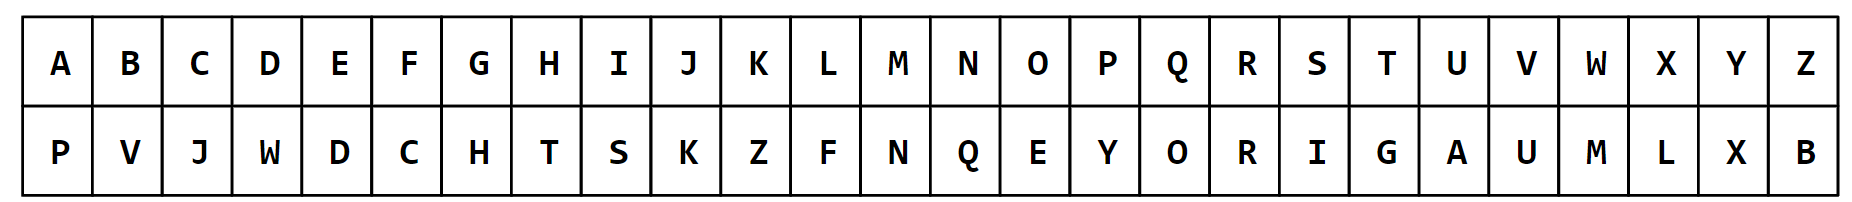
\includegraphics[scale=0.4]{assets/simple_sub.png}
\end{center}
This tells us that 
\begin{itemize}
    \item to \emph{encrypt}, we just need to convert every instance of the top letter to the corresponding bottom letter. For example, encrypting $A$ becomes $P$, encrypting $B$ becomes $V$, and so on.
    \item to \emph{decrypt}, we just need to convert every instance of the bottom letter to the corresponding top letter. For example, decrypting $P$ becomes $A$, decrypting $V$ becomes $B$, and so on.
\end{itemize}
\begin{mdframed}
    (Example.) Suppose Alice wants to encrypt the message \code{You must destroy all of the horcruxes!} She starts by encoding the message\footnote{Removing all spaces, punctuations, and then capitalizing everything.}:
    \begin{verbatim}
YOUMUSTDESTRYALLOFTHEHORCRUXES\end{verbatim}
    Then, she converts each letter using the table: 
    \begin{verbatim}
XEANAIGWDIGREXPFFECGTDTERJRALDI\end{verbatim}
        This is the ciphertext she sends to Bob. To decrypt the message, Bob uses the same table backwards.
\end{mdframed}

Notice that, if the entire table is our key, the number of possible keys is $26!$, a \emph{huge} number. Despite this, simple substitution can still be broken relatively easily using some ideas from probability theory. 

\begin{mdframed}
    (Exercise.) Using the same table given above, do the following by hand. 

    \begin{enumerate}[(a)]
        \item Encrypt the message \code{The moon is pitted with holes!}
        \begin{mdframed}
            Encoding the message gives \code{THEMOONISPITTEDWITHHOLES}. Then, we just need to map each letter appropriately. 
            \begin{verbatim}
plaintext  T H E M O O N I S P I T T E D W I T H H O L E S
ciphertext G T D N E E Q S I Y S G G D W M S G T T E F D I\end{verbatim}
            The answer is \code{GTDNEEQSIYSGGDWMSGTTEFDI}.
        \end{mdframed}

        \item Decrypt the message \code{TEMPRDXEAWESQHGEWPX}.
        \begin{mdframed}
            Mapping each letter appropriately gives us
            \begin{verbatim}
ciphertext T E M P R D X E A W E S Q H G E W P X
plaintext  H O W A R E Y O U D O I N G T O D A Y\end{verbatim}
            Which, decoded, gives us \code{How are you doing today?}
        \end{mdframed}
    \end{enumerate}
\end{mdframed}



\subsection{Polybius Square}
The \textbf{Polybius Square} is another simple substitution cipher which replaces each letter of the plaintext with \emph{two} letters of ciphertext. The idea behind a Polybius square is that it's a table with labeled rows and columns; the alphabet for the messages we're encrypting lives inside the table. For example, if the alphabet we're encrypting includes the capital letters \code{A} through \code{Z} and the digits \code{0} through \code{9}, then we have 36 letters -- perfectly enough to fit in a $6 \times 6$ grid. Consider the following arrangement, using the rows and columns \code{ADFGVX}:
\begin{center}
    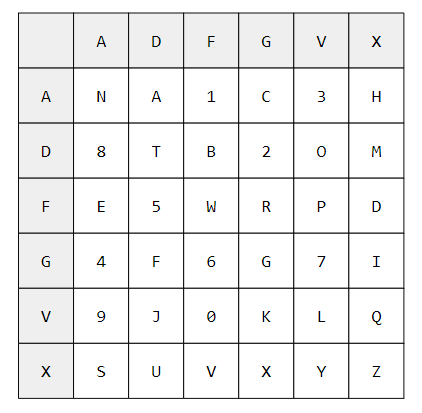
\includegraphics[scale=0.9]{assets/polybius.png}
\end{center}
This table represents our key. To encrypt a message, we convert each letter in the plaintext to a pair of letters indicating the \emph{row} and \emph{column} of that letter in the table above. For example, \code{K} would be replaced with \code{VG}. Similarly, \code{S} would be replaced with \code{XA}. 

\begin{mdframed}
    (Example.) Suppose Alice wants to encrypt the message 
    \begin{verbatim}
Storm the gates at 14:37.\end{verbatim}
    She begins by encoding the message: 
    \begin{verbatim}
STORMTHEGATESAT1437\end{verbatim}
    Then, she goes through and replaces each letter by the corresponding pairs as described above:
    \begin{verbatim}
XADDDVFGDXDDAXFAGGADDDFAXAADDDAFGAAVGV\end{verbatim}
    This is the ciphertext. Bob, who knows the table, can undo this process to decrypt the message. 
\end{mdframed}

\begin{mdframed}
    (Exercise.) Use the square given above.
    \begin{enumerate}[(a)]
        \item Encrypt the message \code{Hide tide at 7:01am}.
        \begin{mdframed}
            Encoding the message gives us \code{HIDETIDEAT701AM}. Then, we can map each individual character in the plaintext to its ciphertext representation:
            \begin{center}
                \begin{tabular}{c|c}
                    \textbf{Plain} & \textbf{Cipher} \\ 
                    \hline 
                    H              & AX \\
                    I              & GX \\
                    G              & GG \\
                    H              & AX \\
                    T              & DD \\
                    I              & GX \\
                    D              & FX \\
                    E              & FA \\
                    A              & AD \\
                    T              & DD \\
                    7              & GV \\
                    0              & VF \\
                    1              & AF \\
                    A              & NN \\
                    M              & DX 
                \end{tabular}
            \end{center}
            Combining all of this gives us 
            \begin{mdframed}
                \begin{verbatim}
AXGXGGAXDDGXFXFAADDDGVVFAFNNDX\end{verbatim}
            \end{mdframed}
        \end{mdframed}
        \item Decrypt the message \code{XAAAADVGFAFVADDDAXADDDDGFVDX}.
        \begin{mdframed}
            To decrypt, we can map each pair of characters in the ciphertext to its plaintext representation:
            \begin{center}
                \begin{tabular}{c|c}
                    \textbf{Cipher} & \textbf{Plain} \\ 
                    \hline 
                    XA              & S \\
                    AA              & N \\
                    AD              & A \\
                    VG              & K \\
                    FA              & E \\
                    FV              & P \\
                    AD              & A \\
                    DD              & T \\
                    AX              & H \\
                    AD              & A \\
                    DD              & T \\
                    DG              & 2 \\
                    FV              & P \\
                    DX              & M 
                \end{tabular} 
            \end{center}
            Combining and decoding gives us 
            \begin{mdframed}
                \begin{verbatim}
Snake path at 2pm\end{verbatim}
            \end{mdframed}
        \end{mdframed}
    \end{enumerate}
\end{mdframed}


\subsection{Interlude: Modular Linear Algebra}
Before going into polygraphic ciphers, let us first discuss how \emph{linear algebra} interacts with modular arithmetic. We'll just work on $2 \times 2$ matrices for now.

\subsubsection{\texorpdfstring{$2 \times 2$ Matrices}{2 by 2 Matrices}}

\begin{definition}{}{}
    A $2 \times 2$ integer \textbf{matrix} (or just \emph{matrix} for short) is a $2 \times 2$ box of numbers $A = \begin{bmatrix}
        a & b \\ c & d
    \end{bmatrix}$ where $a, b, c, d \in \Z$. 
    \begin{itemize}
        \item The \textbf{determinant} of $A$ is the integer $\det(A) = ad - bc$. 
        \item The \textbf{identity matrix} is the matrix $I = \begin{bmatrix}
            1 & 0 \\ 0 & 1
        \end{bmatrix}$. 
        \item Suppose $A = \begin{bmatrix}
            a & b \\ c & d
        \end{bmatrix}$ and $B = \begin{bmatrix}
            a' & b' \\ c' & d'
        \end{bmatrix}$ are two matrices. Their product $AB$ is defined to be \[AB = \begin{bmatrix}
            aa' + bc' & ba' + db' \\ ca' + dc' & cb' + dd'
        \end{bmatrix}.\]
    \end{itemize}
\end{definition}

\begin{mdframed}
    (Example.) Let $A = \begin{bmatrix}
        3 & 2 \\ 1 & 7
    \end{bmatrix}$ and $B = \begin{bmatrix}
        1 & 4 \\ 2 & 3
    \end{bmatrix}$. We know that \[\det(A) = 3 \cdot 7 - 2 \cdot 1 = 19.\] We also know that \[AB = \begin{bmatrix}
        7 & 18 \\ 15 & 25
    \end{bmatrix}\] and \[BA = \begin{bmatrix}
        7 & 30 \\ 9 & 25
    \end{bmatrix}.\] 
\end{mdframed}
\textbf{Remark:} It should be clear from the above example that $AB \neq BA$. That is, matrix multiplication is not commutative. 

\begin{mdframed}
    (Exercise.) Let $A$ be a $2 \times 2$ integer matrix. Show that \[AI = IA = A.\]

    \begin{mdframed}
        Let $A = \begin{bmatrix}
            a & b \\ 
            c & d
        \end{bmatrix}.$ Then, 
        \[IA = \begin{bmatrix}
            1 & 0 \\ 
            0 & 1
        \end{bmatrix} \begin{bmatrix}
            a & b \\ 
            c & d
        \end{bmatrix} = \begin{bmatrix}
            a & b \\ 
            c & d
        \end{bmatrix}\]
        and 
        \[AI = \begin{bmatrix}
            a & b \\ 
            c & d
        \end{bmatrix} \begin{bmatrix}
            1 & 0 \\ 
            0 & 1
        \end{bmatrix} = \begin{bmatrix}
            a & b \\ 
            c & d
        \end{bmatrix}.\]
    \end{mdframed}
\end{mdframed}

\begin{theorem}{Multiplicativity of Determinant}{}
    If $A$ and $B$ are matrices, then $\det(I) = 1$ and \[\det(AB) = \det(A)\det(B).\]
\end{theorem}

\begin{definition}{}{}
    A \textbf{vector} $v$ is a vertical column \[v = \begin{bmatrix}
        x \\ y
    \end{bmatrix},\] where $x, y \in \Z$. 
\end{definition}

\begin{definition}{}{}
    If $A = \begin{bmatrix}
        a & b \\ c & d
    \end{bmatrix}$ is a matrix, then the product $Ab = \begin{bmatrix}
        ax + by \\ 
        cx + dy
    \end{bmatrix}$.
\end{definition}

\subsubsection{Congruences and Inversion for Matrices}
\begin{definition}{}{}
    Fix a positive integer $n$ and suppose $A$ and $B$ are both matrices: 
    \[A = \begin{bmatrix}
        a & b \\ c & d
    \end{bmatrix}, \quad B = \begin{bmatrix}
        a' & b' \\ c' & d'
    \end{bmatrix}.\] We say that $A \equiv B \Mod{n}$ if all four of the entries of the two matrices are congruent mod $n$, i.e., if all of the following are true:  
    \[a \equiv a' \Mod{n}\] 
    \[b \equiv b' \Mod{n}\] 
    \[c \equiv c' \Mod{n}\]
    \[d \equiv d' \Mod{n}\]
\end{definition}

\begin{definition}{}{}
    A matrix $A$ is \emph{invertible mod} $n$ if there exists a matrix $X$ such that $AX \equiv I \Mod{n}$. In this case, $X$ is called an inverse of $A \Mod{n}$. In symbols, we write $X \equiv A^{-1} \Mod{n}$. 
\end{definition}

\begin{theorem}{Modular Inversion Theorem}{}
    Suppose $A = \begin{bmatrix}
        a & b \\ c & d
    \end{bmatrix}$ is a matrix. Then, $A$ is invertible if and only if $\det(A)$ is invertible mod $n$. Moreover, if $e \equiv \det(A)^{-1} \Mod{n}$, then \[X = \begin{bmatrix}
        ed & -eb \\ 
        -ec & ea
    \end{bmatrix}\] is an inverse of $A \Mod{n}$. 
\end{theorem}

\begin{mdframed}
    (Example.) Suppose we have $A = \begin{bmatrix}
        3 & 2 \\ 1 & 7
    \end{bmatrix}$. We know that $\det(A) = 19$ is invertible mod 26, so $A$ is also invertible mod 26. We have \[19^{-1} \equiv 11 \Mod{26},\] so the formula for the inverse from the Matrix Inversion Theorem tells us that \[A^{-1} \equiv \begin{bmatrix}
        11 \cdot 7 & -11 \cdot 2 \\ -11 \cdot 1 & 11 \cdot 3 
    \end{bmatrix} \equiv \begin{bmatrix}
        77 & -22 \\ -11 & 33
    \end{bmatrix} \equiv \begin{bmatrix}
        25 & 4 \\ 15 & 7
    \end{bmatrix} \Mod{26}.\] In other words, \[X = \begin{bmatrix}
        15 & 4 \\ 15 & 7
    \end{bmatrix}\] is an inverse of $A$ mod 26. It follows that $AX = I$. 
\end{mdframed}

\begin{mdframed}
    (Exercise.) Which of the following matrices is invertible mod 26? 
    \begin{enumerate}[(a)]
        \item $\begin{bmatrix}
            7 & 5 \\ 3 & 3 
        \end{bmatrix}$
        \item $\begin{bmatrix}
            8 & 1 \\ 3 & 2 
        \end{bmatrix}$
        \item $\begin{bmatrix}
            4 & 2 \\ 1 & 2 
        \end{bmatrix}$
        \item $\begin{bmatrix}
            4 & 3 \\ 1 & 2
        \end{bmatrix}$
    \end{enumerate}

    \begin{mdframed}
        The answer is \textbf{D}. By calculating the determinant of each matrix, we see that the GCD of the determinant of the matrix and 26 is 1 for only D. 
    \end{mdframed}
\end{mdframed}

\begin{mdframed}
    (Exercise.) As a follow-up to the previous exercise, what is the inverse of the invertible matrix? 

    \begin{mdframed}
        TODO 
    \end{mdframed}
\end{mdframed}

\subsection{Hill Cipher}
The \emph{Hill Cipher} is the first polygraphic cipher we'll talk about. We'll focus on the digraphic case, which replaces 2 letters of plaintext at a time. Our \textbf{key} for this cipher is a matrix that is invertible mod 26. 

\begin{mdframed}
    (Example.) Suppose we want to encrypt the message \textbf{\code{You have saved us all}}. Begin with the usual encoding process: 
    \begin{mdframed}
        \begin{verbatim}
 Y  O  U  H  A  V  E  S  A  V  E  D  U  S  A  L  L
24 14 20  7  0 21  4 18  0 21  4  3 20 18  0 11 11\end{verbatim}
    \end{mdframed} 
    (The numbers below the letters represent the ranking of each letter.) Let's suppose our key is \[A = \begin{bmatrix}
        3 & 2 \\ 1 & 7
    \end{bmatrix},\] which has determinant 19 and is thus invertible mod 26. It follows that $A$ is an invertible matrix mod 26, which can thus be used as a key. 

    \bigskip 

    For encrypting, the idea is to go through the list of numbers, replacing each pair of numbers with the result of multiplying that pair by the matrix $A \Mod{26}$. For example, for the pair 24 and 14, we can make a vector containing these numbers, \[v = \begin{bmatrix}
        24 \\ 14
    \end{bmatrix},\] and then compute \[Av = \begin{bmatrix}
        3 & 2 \\ 1 & 7
    \end{bmatrix} \begin{bmatrix}
        24 \\ 14
    \end{bmatrix} \Mod{26} = \begin{bmatrix}
        100 \\ 122
    \end{bmatrix} \Mod{26} = \begin{bmatrix}
        22 \\ 18
    \end{bmatrix}.\]
    So, we replace the numbers 24 and 14 with the numbers 22 and 18, respectively. In other words, the first two letters of the message will be replaced by \code{W} and \code{S}, respectively. 

    \bigskip 

    We can continue this process with the next pair of numbers (20, 7), and so on. Eventually, we'll reach the end. Note that, if you have an odd number of letters, you can add an additional random letter at the end (e.g., \code{Z}). With this in mind, the net result is the ciphertext
    \begin{mdframed}
\begin{verbatim}
WSWRQRWAQRSZSQWZFE\end{verbatim}
    \end{mdframed}

    As you might expect, to decrypt a message, we just need to multiply the pairs of numbers by the \emph{inverse} of $A$ mod 26.
\end{mdframed}

\begin{mdframed}
    (Exercise.) Use the matrix \[A = \begin{bmatrix}
        3 & -1 \\ 2 & 5
    \end{bmatrix}\] as the key for a Hill cipher. Encrypt the message \code{Go to Lake Lerna}.

    \begin{mdframed}
        First, we verify that this matrix can be used as a key by checking the determinant.
        \[\det(A) = 15 - 2(-1) = 15 + 2 = 17.\]
        Because 17 is invertible mod 26, it follows that we can use $A$ as a key. So, begin by encoding the message: 
        \begin{mdframed}
            \begin{verbatim}
G  O  T  O  L A  K E  L E  R  N A  Z
6 14 19 14 11 0 10 4 11 4 17 13 0 25\end{verbatim}
        \end{mdframed}
        Note that we put a \code{Z} at the end so that the length of the plaintext is even (that way, we can do pairwise encryption.) We'll now process each pair of letters. 
        \begin{itemize}
            \item For pair $(6, 14)$, we have 
            \[\begin{bmatrix}
                3 & -1 \\ 2 & 5
            \end{bmatrix} \begin{bmatrix}
                6 \\ 14
            \end{bmatrix} \Mod{26} = \begin{bmatrix}
                4 \\ 82 
            \end{bmatrix} \Mod{26} = \begin{bmatrix}
                4 \\ 4
            \end{bmatrix},\]
            which corrsponds to \code{E} and \code{E}.

            \item For pair $(19, 14)$, we have 
            \[\begin{bmatrix}
                3 & -1 \\ 2 & 5
            \end{bmatrix} \begin{bmatrix}
                19 \\ 14
            \end{bmatrix} \Mod{26} = \begin{bmatrix}
                43 \\ 108
            \end{bmatrix} \Mod{26} = \begin{bmatrix}
                17 \\ 4
            \end{bmatrix} \Mod{26},\]
            which corresponds to \code{R} and \code{E}.

            \item For pair $(11, 0)$, we have 
            \[\begin{bmatrix}
                3 & -1 \\ 2 & 5
            \end{bmatrix} \begin{bmatrix}
                11 \\ 0
            \end{bmatrix} \Mod{26} = \begin{bmatrix}
                33 \\ 22
            \end{bmatrix} \Mod{26} = \begin{bmatrix}
                7 \\ 22
            \end{bmatrix} \Mod{26},\]
            corresponding to \code{H} and \code{W}.
        \end{itemize}
        By continuing this process, we end up with the ciphertext 
        \begin{mdframed}
\begin{verbatim}
EEREHWAODQMVBV\end{verbatim}
        \end{mdframed}
    \end{mdframed}
\end{mdframed}

\begin{mdframed}
    (Exercise.) Use the matrix \[A = \begin{bmatrix}
        3 & -1 \\ 2 & 5
    \end{bmatrix}\] as the key for a Hill cipher. Decrypt the message \code{RNCQYVFRRLZI}.

    \begin{mdframed}
        Note again that $\det(A) = 17$. In order to decrypt the message, we need to find the inverse of $A$ mod 26.

        \bigskip 

        \textbf{Finding GCD:} Recall that the Matrix Inversion Theorem states that $A$ is invertible if and only if $\det(A)$ is invertible mod $n$. To see if $\det(A)$ is invertible mod $n$, we need to see if $\gcd(\det(A), n) = 1$. So, let's find $\gcd(17, 26)$.  
        \begin{center}
            \begin{tabular}{c|c|c|c|c}
                $a$ & $b$ & $b = aq + r$ & $q$ & $r$ \\ 
                \hline 
                17 & 26 & $26 = 17q + r$ & 1 & 9 \\ 
                9 & 17 & $17 = 9q + r$ & 1 & 8 \\ 
                8 & 9 & $9 = 8q + r$ & 1 & 1 \\ 
                1 & 8 & $8 = 1q + r$ & 8 & 0
            \end{tabular}
        \end{center}
        Therefore, $\gcd(17, 26) = 1$ as desired. Thus, an inverse must exist. 

        \bigskip 
        
        \textbf{Finding Bezout:} Now, we need to find the Bezout coefficients. Labeling each equation, we have 
        \begin{itemize}
            \item (Eq. 1) $26 = 17(1) + 9 \implies 9 = 26 + 17(-1)$ 
            \item (Eq. 2) $17 = 9(1) + 8 \implies 8 = 17 + 9(-1)$
            \item (Eq. 3) $9 = 8(1) + 1 \implies 1 = 9 + 8(-1)$ 
        \end{itemize}
        Now that we've labeled each relevant operation, we can find the Bezout coefficients: 
        \begin{equation*}
            \begin{aligned}
                1 &= 9 + 8(-1) \\ 
                    &= 9 + (\underbrace{17 + 9(-1)}_{\text{Eq. 2}})(-1) \\ 
                    &= 9 + 17(-1) + 9(-1)(-1) \\ 
                    &= 9 + 17(-1) + 9 \\ 
                    &= 9(2) + 17(-1) \\ 
                    &= (\underbrace{26 + 17(-1)}_{\text{Eq. 1}})(2) + 17(-1) \\ 
                    &= 26(2) + 17(-1)(2) + 17(-1) \\ 
                    &= 26(2) + 17(-2) + 17(-1) \\ 
                    &= 26(2) + 17(-3)
            \end{aligned}
        \end{equation*}
        From this, it follows that $x = -3$, which is the desired inverse.  

        \bigskip 

        \textbf{Decrypting:} With this in mind, we have 
        \[X = \begin{bmatrix}
            -3(5) & 3(-1) \\ 3(2) & -3(3)
        \end{bmatrix} = \begin{bmatrix}
            -15 & -3 \\ 6 & -9
        \end{bmatrix} \Mod{26}.\]
        Now that we have the matrix needed to decrypt the message, we can proceed. Labeling each character in the message gives us 
        \begin{mdframed}
            \begin{verbatim}
R  N C  Q  Y  V F  R  R  L  Z I
17 13 2 16 24 21 5 17 17 11 25 8\end{verbatim}
        \end{mdframed}
    \end{mdframed}

    % a pretty stupid hack but at least the frames are readable like this
    \begin{mdframed}
        Iterating over each pair, we have 
        \begin{itemize}
            \item For $(17, 13)$, 
            \[X\begin{bmatrix}
                17 \\ 13
            \end{bmatrix} \Mod{26} = \begin{bmatrix}
                -294 \\ -15
            \end{bmatrix} \Mod{26} = \begin{bmatrix}
                18 \\ 11
            \end{bmatrix} \Mod{26},\]
            or \code{S} and \code{L}. 

            \item For $(2, 16)$, 
            \[X\begin{bmatrix}
                2 \\ 16
            \end{bmatrix} \Mod{26} = \begin{bmatrix}
                -78 \\ -132
            \end{bmatrix} \Mod{26} = \begin{bmatrix}
                0 \\ 24
            \end{bmatrix} \Mod{26},\]
            or \code{A} and \code{Y}.
        \end{itemize}
        By continuing this process, we end up with 
        \begin{mdframed}
            \begin{verbatim}
SLAYTHEHYDRA\end{verbatim}
        \end{mdframed}
    \end{mdframed}
\end{mdframed}

\begin{mdframed}
    (Exercise.) Use the Hill cipher with key \[A = \begin{bmatrix}
        4 & 3 \\ 1 & 2
    \end{bmatrix}\] to encrypt the word \code{AREA}. 

    \begin{mdframed}
        Labeling each letter with its corresponding number, we have 
        \begin{mdframed}
            \begin{verbatim}
0 17 4 0
A  R E A\end{verbatim}
        \end{mdframed}
        Then, we just need to multiply each pair of numbers, like so: 
        \[\begin{bmatrix}
            4 & 3 \\ 1 & 2
        \end{bmatrix} \begin{bmatrix}
            0 \\ 17
        \end{bmatrix} = \begin{bmatrix}
            4 \cdot 0 + 3 \cdot 17 \\ 
            1 \cdot 0 + 2 \cdot 17
        \end{bmatrix} = \begin{bmatrix}
            51 \\ 
            34 
        \end{bmatrix} \equiv \begin{bmatrix}
            25 \\ 
            8
        \end{bmatrix} \Mod{26},\]
        and 
        \[\begin{bmatrix}
            4 & 3 \\ 1 & 2 
        \end{bmatrix} \begin{bmatrix}
            4 \\ 0
        \end{bmatrix} = \begin{bmatrix}
            16 + 0 \\ 
            4 + 0
        \end{bmatrix} \equiv \begin{bmatrix}
            16 \\ 4
        \end{bmatrix} \Mod{26}.\] Therefore, the answer is \code{ZIQE}.
    \end{mdframed}
\end{mdframed}

\begin{mdframed}
    (Exercise.) The matrix \[A = \begin{bmatrix}
        4 & 3 \\ 1 & 2
    \end{bmatrix}\] is used to encrypt \code{CRZX}. What is the plaintext? 

    \begin{mdframed}
        We know that the inverse of $A$ is \[X =  \begin{bmatrix}
            16 & 15 \\ 
            5 & 6 
        \end{bmatrix}.\] Then, going through each pair of numbers gives us 
        \[\begin{bmatrix}
            16 & 15 \\ 5 & 6
        \end{bmatrix} \begin{bmatrix}
            2 \\ 17
        \end{bmatrix} = \begin{bmatrix}
            16 \cdot 2 + 15 \cdot 17 \\ 
            5 \cdot 2 + 6 \cdot 17
        \end{bmatrix} = \begin{bmatrix}
            287 \\ 
            112
        \end{bmatrix} = \begin{bmatrix}
            1 \\ 
            8
        \end{bmatrix},\]
        and 
        \[\begin{bmatrix}
            16 & 15 \\ 5 & 6
        \end{bmatrix} \begin{bmatrix}
            25 \\ 23
        \end{bmatrix} = \begin{bmatrix}
            16 \cdot 25 + 15 \cdot 23 \\ 
            5 \cdot 25 + 6 \cdot 23 
        \end{bmatrix} = \begin{bmatrix}
            745 \\ 263
        \end{bmatrix} \equiv \begin{bmatrix}
            17 \\ 3
        \end{bmatrix}.\]
        This gives us \code{BIRD}.
    \end{mdframed}
\end{mdframed}

\begin{mdframed}
    (Exercise.) Suppose you want to encrypt a sequence of bits (i.e., a sequence of \code{0}'s and \code{1}'s) using a $2 \times 2$ Hill cipher. How many different encryption functions are there? In other words, how many different congruence classes of $2 \times 2$ can be used as a key for a Hill cipher? 

    \begin{mdframed}
        If we assume that our alphabet contains only binary numbers, then there are 2 possible numbers. Therefore, our Hill cipher must be a matrix mod 2. We want to know how many of these matrices are invertible mod 2. 

        \bigskip 

        There are $2 \cdot 2 \cdot 2 \cdot 2$ choices for what our $2 \times 2$ matrix can be. There are three possible determinants: $0$ and $\pm 1$. Note that $-1 \equiv 1 \Mod{2}$ so there's actually \emph{2} possible determinants. Of these determinants, note that $\gcd(1, 2) = 1$ while $\gcd(0, 2) = 2$.
        
        \bigskip 

        With this in mind, we know that any matrix with determinant 1 is valid. There are \boxed{6} such matrices.
    \end{mdframed}
\end{mdframed}

\subsection{Playfair Cipher}
The \textbf{Playfair Cipher} is another digraphic cipher, like the Hill cipher we just discussed above. The key for a Playfair cipher is a $5 \times 5$ grid of letters, where each letter appears exactly once. Because there are 26 letters in the English alphabet but 25 letters can fit in a grid, we treat \code{I} and \code{J} as the same letter\footnote{We could also use a variant where we use a $6 \times 6$ grid that includes all 26 letters and 10 digits, instead.}. 

\bigskip 

How do we start constructing a grid? An easy and convenient way of doing this is to start with a secret keyword. For example, suppose \code{ALPHABET} is our keyword. We can start filling out our grid by writing out the letters of our keyword across the rows, skipping over the letters we've written.
\begin{center}
    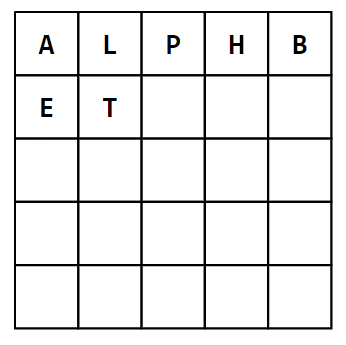
\includegraphics[scale=0.5]{assets/playfair_1.png}
\end{center}
We can then fill out the remaining squares with the remaining letters of the alphabet, skipping over anything we've already written down and remembering that \code{I} and \code{J} are the same. 
\begin{center}
    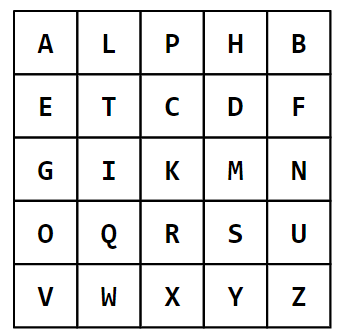
\includegraphics[scale=0.5]{assets/playfair_2.png}
\end{center}
We can encode our message by doing the following: 
\begin{enumerate}
    \item Remove all non-alphabet characters and capitalize everything.
    \item Replace all instances of \code{J} with \code{I}. 
    \item Group the letters into pairs. 
    \item If there are any pairs where both letters are the same, insert the letter \code{X} in between the two letters of that pair and regroup into pairs. 
    \item If there's an unpaired letter at the end, insert the letter \code{X} after it.
\end{enumerate}
\textbf{Remark:} You may need to apply rule 4 multiple times. 

\begin{mdframed}
    (Example.) Suppose we want to encode the message \code{hidden jewels in trees.} Here's what will happen after each step described above. 
    \begin{enumerate}
        \item \code{HIDDENJEWELSINTHETREES}
        \item \code{HIDDENIEWELSINTHETREES}
        \item \code{HI DD EN IE WE LS IN TH ET RE ES}
        \item \code{HI DX DE NI EW EL SI NT HE TR EX ES}
        \item \code{HI DX DE NI EW EL SI NT HE TR EX ES}
    \end{enumerate}
\end{mdframed}

To encrypt, we need to replace each pair with another pair using the grid by following the rules: 
\begin{itemize}
    \item (Row Rule.) If both letters in the pair occur in the same row, replace each letter of the pair with the letter that appears immediately to its right (wrapping around to the left side of the row if needed).
    \item (Column Rule.) If both letters in the pair occur in the same column, replace each letter of the pair with the letter that appears immediately below it (wrapping around to the top of the column if needed).
    \item (Rectangle Rule.) Otherwise, the two letters define a rectangle inside the grid, and we replace each letter with the letter on the same row but the opposite of that rectangle.
\end{itemize}

\begin{mdframed}
    (Example.) Suppose we want to encrypt the message \code{HI DX DE NI EW EL SI NT HE TR EX ES} (see previous example for encoding). Let's look at each pair. 
    \begin{itemize}
        \item For \code{HI}, notice that \code{H} and \code{I} do not appear in the same row or column. Therefore, the rectangle rule applies. Observe the highlighted cells: 
        \begin{center}
            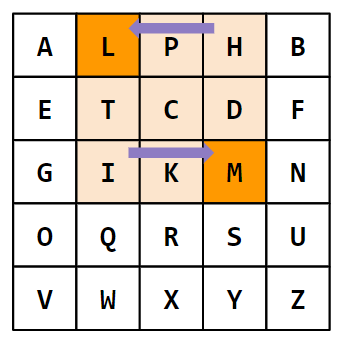
\includegraphics[scale=0.5]{assets/playfair_3.png}
        \end{center}
        Here, the letter in the same row as \code{H} but opposite side is \code{L}, and the letter in the same row as \code{I} but the opposite side is \code{M}. Therefore, \code{HI} becomes \code{LM}. 


        \item For \code{DX}, we also apply the rectangle rule. Observe the highlighted cells: 
        \begin{center}
            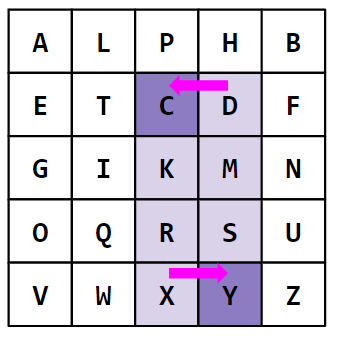
\includegraphics[scale=0.5]{assets/playfair_4.png}
        \end{center}
        So, it follows that \code{DX} gets replaced with \code{CY}.

        \item For \code{DE}, both letters are on the same row so we apply the row rule. Observe that 
        \begin{center}
            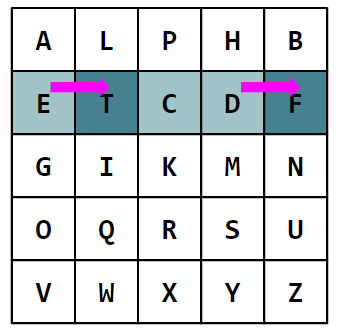
\includegraphics[scale=0.5]{assets/playfair_5.png}
        \end{center}
        So, it follows that \code{DE} becomes \code{FT}.
    \end{itemize}
    Continuing this process yields the desired result.
\end{mdframed}

\begin{mdframed}
    (Exercise.) You are constructing a $5 \times 5$ grid for a Playfair cipher starting with the keyword \code{FAJITAS}. What letter falls in the very center of the grid (i.e., in the 3rd row and the 3rd column)? 

    \begin{enumerate}[(a)]
        \item K
        \item L
        \item M
        \item None of the above. 
    \end{enumerate}

    \begin{mdframed}
        Constructing the grid looks something like: 
        \begin{center}
            \begin{tabular}{|c|c|c|c|c|}
                \hline 
                F & A & I & T & S \\
                \hline 
                B & C & D & E & G \\
                \hline 
                H & K & L & M & N \\
                \hline 
                O & P & Q & R & U \\
                \hline 
                V & W & X & Y & Z \\ 
                \hline 
            \end{tabular}
        \end{center}
        So, the answer is (b). 
    \end{mdframed}
\end{mdframed}

\begin{mdframed}
    (Exercise.) Encode the message \code{Little Fluffy} for encryption using a Playfair cipher. How many pairs of letters are in the encoded message? 

    \begin{enumerate}[(a)]
        \item 6
        \item 7
        \item 8
        \item None of the above. 
    \end{enumerate}

    \begin{mdframed}
        Encoding gives us 
        \begin{itemize}
            \item LITTLEFLUFFY
            \item LITTLEFLUFFY
            \item LITXTLEFLUFXFY
            \item LI TX TL EF LU FX FY
        \end{itemize}
        The answer is (b). 
    \end{mdframed}
\end{mdframed}

\begin{mdframed}
    (Exercise.) Use a Playfair cipher with a key given by the grid below, decrypt \code{WZ LT OP WK SH ES VX PH}.
    \begin{center}
        \begin{tabular}{|c|c|c|c|c|}
            \hline
            C & W & F & Q & Y \\ 
            \hline
            G & I & Z & R & B \\ 
            \hline
            H & M & K & L & U \\ 
            \hline
            V & A & D & E & N \\ 
            \hline
            O & P & X & T & S \\ 
            \hline
        \end{tabular}
    \end{center}

    \begin{mdframed}
        For decryption, we just perform the inverse of the encryption process (e.g., for the row rule, when encrypting is replacing the letter with the one immediately to the right, decrypting is replacing the letter with the one immediately to the left.)
        \begin{itemize}
            \item \code{WZ} maps to \code{FI}.
            \item \code{LT} maps to \code{RE}.
            \item \code{OP} maps to \code{SO}.
            \item \code{WK} maps to \code{FM}.
            \item \code{SH} maps to \code{OU}.
            \item \code{ES} maps to \code{NT}.
            \item \code{VX} maps to \code{DO}.
            \item \code{PH} maps to \code{OM}.
        \end{itemize}
        The answer is \code{FIRESOFMOUNTDOOM}, or \code{Fires of Mount Doom}.
    \end{mdframed}
\end{mdframed}


\subsection{Vigenere Cipher}
The Vigenere cipher is our first example of a \emph{polyalphabetic substitution}, or a substitution cipher in which the substitution scheme changes over the course of the message.

\bigskip 

More specifically, the Vigenere cipher makes use of \emph{modular arithmetic} and the correspondence between the letters \code{A} through \code{Z} and the numbers \code{0} through \code{25}. The \textbf{key} for a Vigenere cipher is a \emph{finite} sequence of shifts. 

\bigskip 

A convenient and, perhaps easy-to-remember, way of constructing such a sequence is to have a secret \emph{keyword}, and then associate each letter of that word with the corresponding number to get the sequence of shift. For example, if our secret keyword is \code{ASGARD}, the corresponding sequence of numbers is $(0, 18, 6, 0, 17, 3)$ because \code{A} corresponds to \code{0}, \code{S} corresponds to \code{18}, and so on.

\begin{mdframed}
    (Example.) Suppose we want to encrypt the message \code{Keep Loki Away}. We begin by encoding the message through the usual way: remove all non-alphabet characters and capitalize everything. 
    \begin{mdframed}
        \code{KEEPLOKIAWAY}
    \end{mdframed}
    Then, we can associate, to each letter in the encoded message, the corresponding numbers 0 through 25.
    \begin{mdframed}
\begin{verbatim}
 K E E  P  L  O  K I A  W A  Y
10 4 4 15 11 14 10 8 0 22 0 24\end{verbatim}
    \end{mdframed}
    We can then perform addition mod 26 to each of these numbers. Specifically, we use the first element of our key sequence for the first number, the second for the second, and so on. When we finish the key, we can just repeat it from the beginning until we're done. From there, we convert those sums back to numbers using te usual correspondence. So, using the key $(0, 18, 6, 0, 17, 3)$ corresponding to the key \code{ASGARD} from above, we have 
    \begin{center}
        \begin{tabular}{c|c c c c c c c c c c c c}
            \textbf{Encoded} & K & E & E & P & L & O & K & I & A & W & A & Y \\ 
            \textbf{Numbers (1)} & 10 & 4 & 4 & 15 & 11 & 14 & 10 & 8 & 0 & 22 & 0 & 24 \\ 
            \textbf{Keyword} & A & S & G & A & R & D & A & S & G & A & R & D \\ 
            \textbf{Key Number (2)} & 0 & 18 & 6 & 0 & 17 & 3 & 0 & 18 & 6 & 0 & 17 & 3 \\ 
            \textbf{(1) + (2) mod 26} & 10 & 22 & 10 & 15 & 2 & 17 & 10 & 0 & 6 & 22 & 17 & 1 \\ 
            \textbf{Encrypted} & K & W & K & P & C & R & K & A & G & W & R & B
        \end{tabular}
    \end{center}
    From this, it follows that \code{KWKPCRKAGWRB} is the ciphertext.
\end{mdframed}
\textbf{Remarks:}
\begin{itemize}
    \item As mentioned earlier, the Vigenere cipher is polyalphabetic. Notice how the first \code{E} in the example above was encrypted to \code{W}, whilethe second \code{E} was encrypted to \code{K}. 
    \item For decryption, the process is nearly the same. The only difference is that we \emph{subtract} mod 26 instead of add. 
\end{itemize} 

\begin{mdframed}
    (Exercise.) Using the keyword \code{ASGARD}, 
    \begin{itemize}
        \item Encrypt the message \code{Protect Odin from Fenrir}.
        \begin{mdframed}
            Encoding the message gives us \code{PROTECTODINFROMFENRIR}. From there, we can label each letter:
            \begin{mdframed}
                \begin{verbatim}
 P  R  O  T E C  T  O D I  N F  R  O  M F E  N  R I  R
15 17 14 19 4 2 19 14 3 8 13 5 17 14 12 5 4 13 17 8 17\end{verbatim}
            \end{mdframed}
            Noting that the key, \code{ASGARD}, has numerical correspondence $(0, 18, 6, 0, 17, 3)$, we can run through the encryption process: 
            \begin{mdframed}
\begin{verbatim}
Encoded            P  R  O  T  E  C  T  O  D  I  N
Numbers (1)        15 17 14 19 4  2  19 14 3  8  13 
Keyword            A  S  G  A  R  D  A  S  G  A  R
Key Numbers (2)    0  18 6  0  17 3  0  18 6  0  17
(1) + (2) mod 26   15 9  20 19 21 5  19 6  9  8  4
Encrypted          P  J  U  T  V  F  T  G  J  I  E

Encoded            F  R  O  M  F  E  N  R  I  R
Numbers (1)        5  17 14 12 5  4  13 17 8  17
Keyword            D  A  S  G  A  R  D  A  S  G
Key Numbers (2)    3  0  18 6  0  17 3  0  18 6
(1) + (2) mod 26   8  17 6  18 5  21 16 17 0  23
Encrypted          I  R  G  S  F  V  Q  R  A  X\end{verbatim}
            \end{mdframed}
            This yields the ciphertext 
            \begin{mdframed}
                \code{PJUTVFTGJIEIRGSFVQRAX}.
            \end{mdframed}
        \end{mdframed}

        \item Decrypt the message \code{RSMNRUOCOSTRMATG}.
        \begin{mdframed}
            We begin by labeling each letter: 
            \begin{mdframed}
                \begin{verbatim}
 R  S  M  N  R  U  O C  O  S  T  R  M A  T G
17 18 12 13 17 20 14 2 14 18 19 17 12 0 19 6\end{verbatim}
            \end{mdframed}
            From there, we can run through the decryption process: 
            \begin{mdframed}
\begin{verbatim}
Encoded            R  S  M  N  R  U  O  C  O  S  T  R  M  A  T  G
Numbers (1)        17 18 12 13 17 20 14 2  14 18 19 17 12 0  19 6
Keyword            A  S  G  A  R  D  A  S  G  A  R  D  A  S  G  A 
Key Numbers (2)    0  18 6  0  17 3  0  18 6  0  17 3  0  18 6  0 
(1) - (2) mod 26   17 0  6  13 0  17 14 10 8  18 2  14 12 8  13 6
Decrypted          R  A  G  N  A  R  O  K  I  S  C  O  M  I  N  G\end{verbatim}
            \end{mdframed}
            Decoding the message yields
            \begin{mdframed}
                \code{Ragnarok is coming} 
            \end{mdframed}
        \end{mdframed}
    \end{itemize}
\end{mdframed}

\begin{mdframed}
    (Exercise.) Use a Vigenere cipher with keyword \code{AND} to encrypt the message \code{Six Meals}. 

    \begin{mdframed}
        Encoding and mapping each letter to the corresponding number, we have 
        \begin{mdframed}
            \begin{verbatim}
S  I  X  M  E  A  L  S
18 8  23 12 4  0  11 18\end{verbatim}
        \end{mdframed}

        From there, we can run through the encryption process: 
        \begin{mdframed}
            \begin{verbatim}
Encoded             S  I  X  M  E  A  L  S
Numbers (1)         18 8  23 12 4  0  11 18
Keyword             A  N  D  A  N  D  A  N
Key Numbers (2)     0  13 3  0  13 3  0  13
(1) + (2) mod 26    18 21 0  12 17 3  11 5
Encrypted           S  V  A  M  R  D  L  F\end{verbatim}
        \end{mdframed}
        Therefore, the answer is \code{SVAMRDLF}.
    \end{mdframed}
\end{mdframed}

\begin{mdframed}
    (Exercise.) Use a Vigenere cipher with keyword \code{AND} to decrypt \code{YEX SUD LYQ OGS AFV}. 

    \begin{mdframed}
        Running through the decryption process yields 
        \begin{mdframed}
\begin{verbatim}
Encoded             Y  E  X  S  U  D  L  Y  Q  O  G  S  A  F  V 
Numbers (1)         24 1  23 18 20 3  11 24 16 14 6  18 0  5  21
Keyword             A  N  D  A  N  D  A  N  D  A  N  D  A  N  D
Key Numbers         0  13 3  0  13 3  0  13 3  0  13 3  0  13 3
(1) - (2) mod 26    24 14 20 18 7  0  11 11 13 14 19 15 0  18 18
Decrypted           Y  O  U  S  H  A  L  L  N  O  T  P  A  S  S 
\end{verbatim}
        \end{mdframed}
        This yields \code{YOUSHALLNOTPASS}, or \code{You shall not pass}.
    \end{mdframed}
\end{mdframed}

\subsection{One-Time Pad}
The \emph{one-time pad} is a special case of the Vigenere cipher where the key sequence is 
\begin{itemize}
    \item never re-used, 
    \item at least as long as the plaintext, 
    \item ``unrelated to the plaintext,'' and 
    \item ``totally random,'' in the sense that each number 0 through 25 is equally likely in each position of the key.
\end{itemize}
Essentially, the way the one-time pad functions is very similar to the Vigenere cipher, except that the key sequence must not be generated using a keyword\footnote{The issue with this is that words won't have the property that each letter is equally likely.}. 

\bigskip 

In any case, we'll revisit this section later -- it's important to be precise when talking about what ``unrelated to the plaintext'' and ``totally random'' means. We'll also see, later on, that this has a property known as \emph{perfect secrecy}, which means that the security of the one-time pad can be mathematically guaranteed. 

\end{document}